\documentclass[12pt,a4paper,twoside]{article}

\usepackage{fontspec}
\setmainfont{Calibri}
\setsansfont{Calibri}
\usepackage[romanian]{babel}
\usepackage[a4paper,margin=2.5cm]{geometry}
\usepackage{fancyhdr}
\usepackage{graphicx}
\usepackage{float}
\usepackage{textcomp}
\usepackage{array}
\usepackage{booktabs}
\usepackage{longtable}
\usepackage{enumitem}
\usepackage{titlesec}
\usepackage{parskip}
\usepackage[hidelinks]{hyperref}
\usepackage{tikz}
\usetikzlibrary{positioning, arrows.meta, shapes.geometric, fit, calc, backgrounds}
\usepackage{pdfpages}

\titleformat{\section}{\Large\bfseries}{\thesection}{0.7em}{}
\titleformat{\subsection}{\large\bfseries}{\thesubsection}{0.7em}{}
\titleformat{\subsubsection}{\normalsize\bfseries}{\thesubsubsection}{0.7em}{}
\titlespacing*{\section}{0pt}{2.2ex plus 1ex minus .2ex}{1.4ex plus .2ex}
\titlespacing*{\subsection}{0pt}{1.8ex plus 1ex minus .2ex}{1.0ex plus .2ex}
\titlespacing*{\subsubsection}{0pt}{1.4ex plus 1ex minus .2ex}{0.8ex plus .2ex}

\setcounter{secnumdepth}{3}
\setcounter{tocdepth}{3}

\pagestyle{fancy}
\fancyhf{}
\fancyhead[RE,LO]{\small Stancu Nicol-Alexia}
\fancyfoot[C]{\thepage}
\renewcommand{\headrulewidth}{0.4pt}

\newcommand{\spo}{SpO\textsubscript{2}}

\newcommand{\figplaceholder}[1]{\fbox{\parbox[c][4.8cm][c]{0.88\textwidth}{\centering\itshape #1}}}

\addto\captionsromanian{\renewcommand{\refname}{Bibliografie}}

\setlength{\parskip}{0.6em}
\renewcommand{\baselinestretch}{1.0}  % spațiere la un rând

\begin{document}

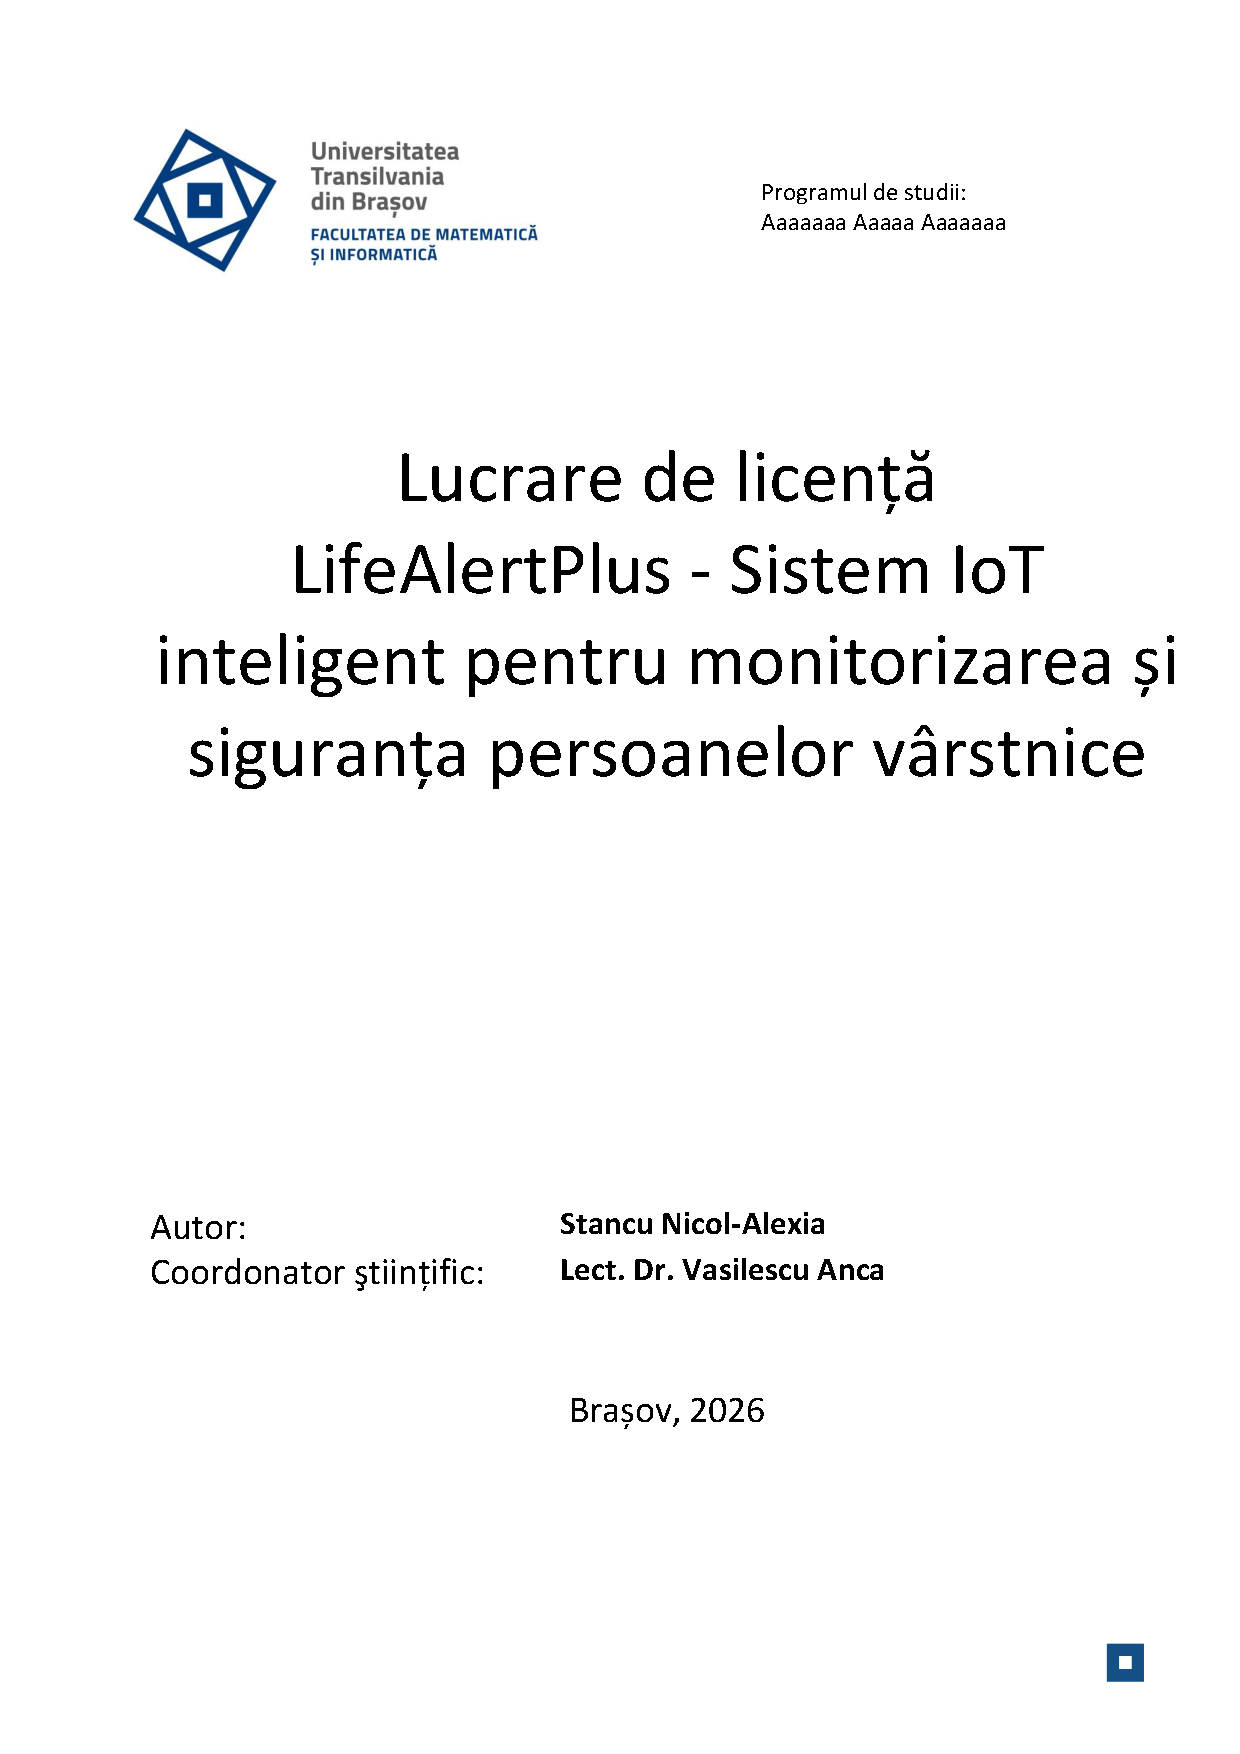
\includepdf[pages=-]{coperta-partea1.pdf}

\newpage
\tableofcontents
\newpage

\phantomsection
\addcontentsline{toc}{section}{Listă de figuri}
\listoffigures
\newpage

\phantomsection
\addcontentsline{toc}{section}{Listă de tabele}
\listoftables
\newpage

\phantomsection
\addcontentsline{toc}{section}{Listă de abrevieri}
\section*{Listă de abrevieri}

{\small
\renewcommand{\arraystretch}{1.25}
\begin{longtable}{@{}>{\bfseries}p{2.7cm}p{10.6cm}@{}}
AI & Artificial Intelligence, în traducere inteligență artificială\\
API & Application Programming Interface, interfață de programare a aplicațiilor\\
AUC-ROC & Area Under the ROC Curve, aria de sub curba ROC\\
AV & Alură ventriculară (frecvență cardiacă)\\
BIDMC & Beth Israel Deaconess Medical Center, instituție sursă a unui set public de date fiziologice\\
BLE & Bluetooth Low Energy\\
bpm & Bătăi pe minut (unitate pentru frecvența cardiacă)\\
CI/CD & Continuous Integration / Continuous Delivery, adică integrare și livrare continuă\\
CORS & Cross-Origin Resource Sharing\\
CPaaS & Communication Platform as a Service, platformă de comunicație în cloud\\
DTO & Data Transfer Object, obiect de transfer de date\\
ECG & Electrocardiogramă\\
EDA & Electrodermal Activity, activitate electrodermală\\
ESP-IDF & Espressif IoT Development Framework, mediul de dezvoltare pentru microcontrollere Espressif\\
FreeRTOS & Free Real-Time Operating System, sistem de operare în timp real\\
GPIO & General-Purpose Input/Output, pin de intrare/ieșire de uz general\\
GPS & Global Positioning System, sistem de poziționare globală\\
HTTP & HyperText Transfer Protocol\\
HTTPS & HyperText Transfer Protocol Secure, adică HTTP securizat\\
I2C & Inter-Integrated Circuit, magistrală de comunicație serială\\
IMU & Inertial Measurement Unit, unitate de măsurare inerțială\\
IoMT & Internet of Medical Things, internetul dispozitivelor medicale\\
IoT & Internet of Things, internetul lucrurilor\\
JSON & JavaScript Object Notation, format de schimb de date\\
JWT & JSON Web Token\\
LED & Light-Emitting Diode, diodă electroluminescentă\\
LiPo & Lithium Polymer, acumulator litiu-polimer\\
MQTT & Message Queuing Telemetry Transport, protocol de comunicație IoT\\
NMEA & National Marine Electronics Association, standard de format pentru datele GPS\\
NVS & Non-Volatile Storage, memorie nevolatilă\\
OAuth & Open Authorization, protocol de autorizare delegată\\
OLED & Organic Light-Emitting Diode, ecran cu diode electroluminescente organice\\
ORM & Object-Relational Mapper, mapare obiect-relațional\\
PERS & Personal Emergency Response System, sistem de alertă personală medicală\\
PPG & Photoplethysmography, fotopletismografie\\
PWA & Progressive Web Application, aplicație web progresivă\\
REST & Representational State Transfer, stil arhitectural pentru API-uri web\\
RFID & Radio-Frequency Identification, identificare prin radiofrecvență\\
RISC-V & Reduced Instruction Set Computer, arhitectură deschisă de procesor\\
ROC & Receiver Operating Characteristic, curbă de evaluare a clasificatorilor\\
SHAP & SHapley Additive exPlanations, metodă de explicare a modelelor de inteligență artificială\\
SMS & Short Message Service, serviciu de mesaje text\\
SMTP & Simple Mail Transfer Protocol, protocol de trimitere a email-urilor\\
SPA & Single-Page Application, aplicație web cu pagină unică\\
SPI & Serial Peripheral Interface, magistrală de comunicație serială\\
\spo & Saturația periferică a oxigenului în sânge\\
TLS & Transport Layer Security, protocol de securizare a comunicației\\
TTFF & Time To First Fix, timpul până la primul fix GPS\\
UART & Universal Asynchronous Receiver-Transmitter, interfață de comunicație serială\\
USB-C & Universal Serial Bus Type-C\\
WiFi & Tehnologie de rețea locală fără fir (standard IEEE 802.11)\\
OTA & Over-The-Air, actualizare de firmware fără conexiune fizică\\
VAPID & Voluntary Application Server Identification, standard de autentificare pentru Web Push\\
WDT & Watchdog Timer, circuit de supraveghere a buclei principale\\
\end{longtable}
}
\addtocounter{table}{-1}

\newpage

\section{Introducere}

\subsection{Context actual}

Transformarea digitală a sistemelor de sănătate reprezintă una dintre tendințele cele mai semnificative ale ultimului deceniu. La nivel global, numărul persoanelor diagnosticate cu afecțiuni cronice precum diabetul, hipertensiunea sau bolile cardiovasculare depășește 1,9 miliarde, potrivit datelor Organizației Mondiale a Sănătății (2023). În România, aproximativ 35\% din populație suferă de cel puțin o boală cronică, un procentaj care pune o presiune considerabilă asupra sistemului medical tradițional, bazat în principal pe consultații periodice și internări.

O categorie deosebit de vulnerabilă o constituie \textbf{persoanele vârstnice}: în România, populația cu vârsta de peste 65 de ani reprezintă aproximativ 20\% din total, iar proiecțiile demografice indică o creștere semnificativă a acestei ponderi în deceniile următoare. Vârstnicii sunt predispuși la afecțiuni cronice multiple, la căderi accidentale și la episoade acute care, nedepistate la timp, pot pune viața în pericol. Caracterul lor adesea singuratic și dificultatea de a accesa prompt serviciile medicale sporesc riscul ca o situație critică să treacă neobservată ore sau zile întregi.

În acest context, tehnologiile Internet of Things (IoT) oferă o alternativă viabilă: monitorizarea continuă a pacienților în afara mediului spitalicesc, prin intermediul senzorilor portabili capabili să măsoare parametri vitali precum ritmul cardiac, saturația oxigenului în sânge (\spo) și temperatura corporală, dar și să detecteze, prin senzori de mișcare, evenimente critice precum căderile. Datele colectate sunt transmise în timp real către platforme software care le procesează, le stochează și le analizează, permițând intervenția rapidă a aparținătorilor sau a serviciilor de urgență.

Această abordare reduce costurile de spitalizare, crește autonomia vârstnicului și îmbunătățește calitatea actului medical prin accesul la date obiective și continue.

\subsection{Motivația alegerii temei}

Alegerea acestei teme a fost motivată de dorința de a dezvolta o soluție tehnologică cu impact direct și măsurabil asupra calității vieții utilizatorilor. Sistemele de monitorizare existente sunt adesea costisitoare, greu de configurat sau limitate la mediul clinic, ceea ce le face inaccesibile pentru utilizatorul obișnuit.

Provocarea de a integra mai multe tehnologii moderne, precum senzori IoT, comunicație wireless, backend scalabil, aplicație web și mecanisme de notificare prin SMS, email și notificări push, a reprezentat un factor motivant suplimentar. Complexitatea tehnică a proiectului oferă oportunitatea aplicării practice a cunoștințelor acumulate pe parcursul studiilor, într-un scenariu cu relevanță reală.

Nu în ultimul rând, posibilitatea de a defini și implementa un mecanism propriu de evaluare a stării de sănătate a utilizatorului, denumit în lucrare \textit{health score}, a constituit o motivație importantă, reprezentând o contribuție originală față de soluțiile existente.

\subsection{Scopul lucrării}

Scopul lucrării este de a demonstra că un sistem IoT de monitorizare medicală accesibil, fiabil și scalabil poate fi proiectat și implementat cu tehnologii open-source și hardware de uz general, fără a necesita infrastructură specializată de nivel clinic.

Dincolo de aspectul tehnic, lucrarea urmărește să arate că o astfel de soluție poate contribui la prevenirea complicațiilor medicale prin detectarea timpurie a anomaliilor și notificarea automată a persoanelor responsabile, fie ele aparținători, medici sau servicii de urgență. În situațiile critice, intervenția rapidă este sprijinită de localizarea GPS a pacientului și de un buton de panică prin care acesta poate solicita direct ajutor.

\subsection{Obiective}

Pentru realizarea scopului propus, au fost stabilite următoarele obiective:

\textbf{O1}: proiectarea și implementarea unui subsistem de achiziție a datelor de la senzori biomedicali (ritm cardiac, \spo, temperatură corporală) și de la un senzor inerțial pentru detectarea mișcării și a căderilor, precum și a poziției geografice prin GPS, cu transmitere în timp real către un server centralizat.

\textbf{O2}: dezvoltarea unei aplicații web pentru vizualizarea datelor colectate, accesibilă persoanelor responsabile de monitorizare.

\textbf{O3}: definirea și implementarea unui mecanism inteligent de evaluare a stării de sănătate, care combină un model de învățare automată pentru clasificarea stării pacientului cu un indice sintetic original (health score), bazat pe corelarea mai multor parametri vitali și pe praguri de alertă personalizabile.

\textbf{O4}: integrarea unui sistem de notificări multi-canal (SMS, email, notificări push) care să fie declanșat automat atunci când health score-ul coboară sub un prag critic.

\textbf{O5}: asigurarea funcționării sistemului în timp real, cu latență minimă între achiziția datelor și afișarea/alertarea acestora.

\textbf{O6}: proiectarea unei arhitecturi modulare și scalabile, capabile să susțină un număr crescut de utilizatori și dispozitive fără modificări structurale majore.

\subsection{Contribuții personale}

Lucrarea de față aduce următoarele contribuții originale:

\textbf{Arhitectura sistemului}: a fost proiectată integral de autor, alegând o structură modulară care separă clar nivelul de achiziție (dispozitiv IoT), nivelul de procesare (backend) și nivelul de prezentare (frontend), facilitând astfel întreținerea și extinderea ulterioară.

\textbf{Mecanismul health score}: reprezintă contribuția cu cel mai înalt grad de originalitate. Spre deosebire de sistemele existente care alertează pe baza depășirii unui singur prag (ex: AV > 100 bpm), health score-ul propus corelează simultan mai mulți parametri vitali, ponderați în funcție de severitate, producând un indice unic al stării de sănătate, mai expresiv și mai puțin predispus la alerte false.

\textbf{Modelul de inteligență artificială}: a fost antrenat și integrat un model de învățare automată (Random Forest) pentru clasificarea automată a stării de sănătate în categoriile normal, alertă și critic. Modelul este combinat cu un set de reguli medicale într-un mecanism hibrid de decizie și este expus printr-un microserviciu dedicat.

\textbf{Implementarea backend și frontend}: întreaga aplicație software a fost dezvoltată de autor, inclusiv API-ul REST pentru comunicarea cu dispozitivele IoT, baza de date pentru stocarea istoricului și interfața web pentru vizualizare.

\textbf{Integrarea senzorilor}: configurarea și calibrarea senzorilor pentru achiziția corectă a datelor biomedicale, precum și implementarea protocolului de comunicație dintre dispozitiv și server.

\textbf{Stocarea locală și sincronizarea datelor}: pentru a asigura continuitatea înregistrării chiar și în absența conexiunii la internet, dispozitivul stochează temporar măsurătorile într-o coadă locală și le sincronizează automat cu serverul la revenirea semnalului.

\textbf{Sistemul de alertare multi-canal}: proiectarea logicii de declanșare a notificărilor și integrarea serviciilor externe pentru livrarea acestora prin SMS, email și notificări push.

\subsection{Structura lucrării}

Lucrarea este organizată în șapte capitole, fiecare tratând un aspect distinct al dezvoltării sistemului.

Capitolul II prezintă fundamentele teoretice necesare înțelegerii lucrării: concepte IoT, protocoale de comunicație, senzori biomedicali și tehnologii software utilizate.

Capitolul III analizează critic soluțiile existente pe piață și în literatura de specialitate, identificând limitările acestora și justificând abordarea propusă.

Capitolul IV descrie proiectarea sistemului, anume arhitectura generală, fluxul de date, structura bazei de date și logica mecanismului health score.

Capitolul V detaliază implementarea efectivă a fiecărei componente: firmware-ul dispozitivului IoT, backend-ul, frontend-ul și sistemul de notificări.

Capitolul VI prezintă metodologia de testare și rezultatele obținute, cu accent pe acuratețea datelor, latența sistemului și fiabilitatea alertelor.

Capitolul VII formulează concluziile lucrării, limitările identificate și direcțiile de dezvoltare ulterioară.

\newpage
\section{Fundamente teoretice și tehnologii}

\subsection{Internet of Things}

Termenul Internet of Things (IoT) descrie un ecosistem de dispozitive fizice echipate cu senzori, procesoare și module de comunicație, capabile să colecteze și să schimbe date prin intermediul rețelelor de comunicații, fără a necesita intervenție umană directă. Conceptul a fost introdus pentru prima dată de Kevin Ashton în 1999, în contextul identificării prin radiofrecvență (RFID), și s-a extins ulterior pentru a descrie orice obiect conectat la internet capabil să interacționeze cu mediul înconjurător.

Din punct de vedere arhitectural, un sistem IoT este organizat pe trei niveluri principale. Primul nivel, numit nivelul de percepție, cuprinde dispozitivele fizice și senzorii responsabili de achiziția datelor din mediu. Al doilea nivel, nivelul de rețea, asigură transmiterea datelor colectate către infrastructura de procesare, utilizând protocoale precum WiFi, Bluetooth Low Energy (BLE), MQTT sau HTTP. Al treilea nivel, nivelul de aplicație, include platformele software care procesează, stochează și prezintă datele utilizatorilor finali.

În domeniul medical, IoT a generat un subdomeniu distinct, denumit Internet of Medical Things (IoMT), care cuprinde dispozitive precum brățări de monitorizare, pulsioximetre portabile, glucometre conectate și sisteme de monitorizare a semnelor vitale. Potrivit unui raport Fortune Business Insights din 2023, piața globală IoMT a depășit 50 de miliarde de dolari și este estimată să crească la peste 180 de miliarde până în 2030, reflectând cererea crescândă pentru soluții de monitorizare continuă în afara mediului clinic.

Un aspect critic în sistemele IoT medicale este fiabilitatea comunicației. Spre deosebire de aplicațiile industriale sau de automatizare casnică, întreruperea transmisiei datelor într-un sistem medical poate avea consecințe directe asupra siguranței pacientului. Din acest motiv, arhitecturile IoMT includ în mod obișnuit mecanisme de stocare locală temporară a datelor, care asigură continuitatea înregistrării chiar și în absența conectivității la rețea, cu sincronizare automată la revenirea conexiunii.

În cadrul sistemului dezvoltat în această lucrare, arhitectura IoT este implementată pe trei niveluri corespunzătoare: un dispozitiv portabil bazat pe microcontrollerul ESP32-C3 Mini în rolul de nod de percepție, comunicația WiFi în rolul nivelului de rețea, și o aplicație web deployată pe Azure în rolul nivelului de aplicație. Dat fiind că sistemul este destinat persoanelor vârstnice, s-a acordat o atenție deosebită simplificării interacțiunii cu dispozitivul, configurarea tehnică fiind realizată o singură dată de aparținător, iar funcționarea ulterioară fiind complet transparentă pentru pacient. Corespondența între cele trei niveluri teoretice și componentele concrete ale sistemului este ilustrată în figura~\ref{fig:iot-layers}.

\begin{figure}[H]
\centering
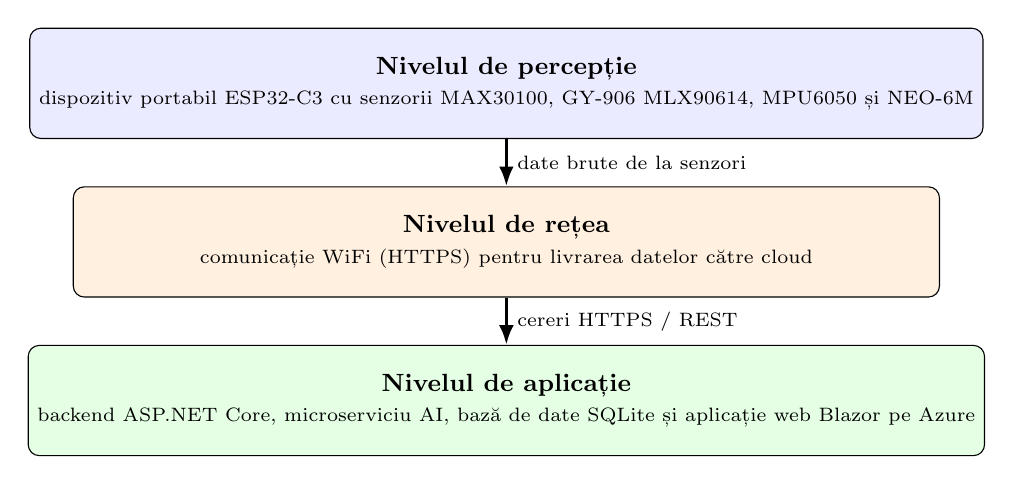
\begin{tikzpicture}[node distance=0.6cm and 1.2cm,
    every node/.style={font=\small},
    layer/.style={rectangle, rounded corners, draw, minimum width=11cm, minimum height=1.4cm, align=center},
    perc/.style={layer, fill=blue!8},
    ret/.style={layer, fill=orange!12},
    app/.style={layer, fill=green!10},
    arrow/.style={-{Latex[length=2.5mm]}, very thick}]

  \node[perc] (perc) {\textbf{Nivelul de percepție}\\\scriptsize dispozitiv portabil ESP32-C3 cu senzorii MAX30100, GY-906 MLX90614, MPU6050 și NEO-6M};
  \node[ret, below=of perc] (ret) {\textbf{Nivelul de rețea}\\\scriptsize comunicație WiFi (HTTPS) pentru livrarea datelor către cloud};
  \node[app, below=of ret] (app) {\textbf{Nivelul de aplicație}\\\scriptsize backend ASP.NET Core, microserviciu AI, bază de date SQLite și aplicație web Blazor pe Azure};

  \draw[arrow] (perc) -- node[right, font=\scriptsize]{date brute de la senzori} (ret);
  \draw[arrow] (ret) -- node[right, font=\scriptsize]{cereri HTTPS / REST} (app);
\end{tikzpicture}
\caption{Cele trei niveluri ale arhitecturii IoT și corespondența lor în sistemul LifeAlertPlus.}
\label{fig:iot-layers}
\end{figure}

\subsection{Senzori și dispozitive}

\subsubsection{Microcontrollerul ESP32-C3 Mini}

ESP32-C3 Mini este un microcontroller de dimensiuni reduse, produs de Espressif Systems, bazat pe arhitectura RISC-V pe 32 de biți. Dispune de conectivitate WiFi 802.11 b/g/n și Bluetooth 5.0 Low Energy, ceea ce îl face potrivit pentru aplicații IoT portabile care necesită atât comunicație locală, cât și acces la internet. Consumul redus de energie, dimensiunile compacte și suportul pentru protocoale de comunicație standard precum I2C, SPI și UART îl recomandă ca platformă centrală pentru un dispozitiv de tip brățară medicală.

În cadrul sistemului, ESP32-C3 Mini îndeplinește rolul de unitate centrală de procesare a dispozitivului portabil: colectează datele de la toți senzorii, le procesează local, le afișează pe ecranul OLED și le transmite către serverul din cloud prin WiFi.

\subsubsection{Senzorul MAX30100 pentru puls și saturație de oxigen}

MAX30100 este un senzor optic integrat, produs de Maxim Integrated, destinat măsurării neinvazive a frecvenței cardiace și a saturației oxigenului în sânge (\spo). Funcționarea sa se bazează pe principiul \textbf{fotopletismografiei (PPG)}: senzorul emite lumină în spectrul roșu și infraroșu prin țesutul cutanat, iar un fotodetector măsoară variațiile de absorbție cauzate de pulsațiile sângelui. Diferența de absorbție dintre hemoglobina oxigenată și cea dezoxigenată permite calcularea \spo.

Comunicația cu microcontrollerul se realizează prin protocolul \textbf{I2C}, la o adresă fixă de 0x57. Tensiunea de alimentare este de 1.8V pentru nucleul digital și 3.3V pentru LED-uri, necesitând atenție la proiectarea schemei electrice. Valorile normale ale parametrilor măsurați sunt între 60 și 100 bătăi pe minut pentru frecvența cardiacă și între 95\% și 100\% pentru \spo, valorile sub 90\% indicând o hipoxemie potențial critică.

\subsubsection{Senzorul GY-906 MLX90614 pentru temperatura corporală}

GY-906 MLX90614 este un senzor infraroșu \textbf{fără contact} pentru măsurarea temperaturii, produs de Melexis, capabil să măsoare temperatura obiectului vizat fără a necesita atingerea acestuia. Senzorul conține atât un termometru infraroșu pentru obiect (câmpul de vizionare 90°), cât și un senzor de temperatură ambiantă, ceea ce permite compensarea temperaturii mediului. Comunicația cu microcontrollerul se realizează prin protocolul \textbf{I2C} (adresă implicită 0x5A), ceea ce permite conectarea senzorului la magistrala comună gestionată de multiplexorul TCA9548A.

Precizia de $\pm$0.5\textdegree C în intervalul clinic relevant (36--42\textdegree C) îl face adecvat pentru detectarea temperaturii corporale fără contact. Intervalul de măsurare pentru obiect este de -70\textdegree C până la +380\textdegree C, iar cel pentru temperatura ambiantă de -40\textdegree C până la +125\textdegree C. Consumul de curent este de aproximativ 1.5\,mA în mod activ. Avantajul principal pentru aplicația de față este că măsurătoarea se realizează \textbf{fără contact direct cu pielea}, eliminând disconfortul purtătorului și riscul de contaminare creuciată.

\subsubsection{Senzorul MPU6050 pentru mișcare și accelerație}

MPU6050, produs de InvenSense, este o unitate de măsurare inerțială (IMU) care integrează un accelerometru triaxial și un giroscop triaxial într-un singur circuit, comunicând prin \textbf{I2C} la adresele 0x68 sau 0x69. Accelerometrul măsoară accelerația pe axele X, Y și Z, iar giroscopul măsoară viteza unghiulară, permițând împreună determinarea orientării și a tipului de mișcare al purtătorului.

În contextul acestei lucrări, datele furnizate de MPU6050 sunt utilizate în două scopuri distincte. Primul scop este \textbf{detectarea activității fizice} (mers, repaus, somn), pentru construirea profilului de activitate zilnică al pacientului. Al doilea scop, cu implicații directe asupra siguranței, este \textbf{detectarea căderilor}, un eveniment frecvent și potențial grav în cazul persoanelor vârstnice. Algoritmul de detecție folosește un detector clasic bazat pe praguri aplicate magnitudinii acceleraţiei: o cădere reală combină o scurtă perioadă de \textit{free-fall} (magnitudine sub aproximativ 0,5\,g), un \textit{impact} brusc (magnitudine peste 2,5\,g) și o perioadă ulterioară de \textit{imobilitate} a pacientului (variaţii mici în jurul valorii de 1\,g). Implementarea concretă a acestui algoritm, ca task FreeRTOS dedicat pe microcontroller, este detaliată în subcapitolul 5.1.

Interpretarea datelor brute ale senzorului pentru clasificarea activităților este realizată de un modul AI descris în subcapitolul 2.3.

\subsubsection{Modulul GPS NEO-6M}

NEO-6M este un modul GPS produs de u-blox, capabil să determine poziția geografică cu o precizie de aproximativ 2.5 metri în condiții favorabile. Comunicația cu microcontrollerul se realizează prin \textbf{UART}, la o rată de 9600 baud implicit, transmițând date în format NMEA 0183. Timpul de achiziție a primului fix GPS (TTFF) este de aproximativ 27 de secunde la pornire rece și sub 1 secundă la pornire caldă.

O limitare importantă a modulului GPS este că semnalul satelitar \textbf{nu este disponibil în interiorul clădirilor}, în subsoluri sau în zone cu vizibilitate redusă a cerului (zone urbane dens construite, vehicule cu geamuri termoizolante). În aceste condiții frecvente în contextul monitorizării vârstnicilor la domiciliu, modulul nu poate furniza coordonate valide, iar câmpul de localizare rămâne nul în datele transmise. Firmware-ul gestionează această situație printr-un mecanism de timeout de 5 minute: dacă nu se obține niciun fix valid, driverul UART este oprit temporar pentru a economisi curentul consumat (~30\,mA).

În cadrul sistemului, modulul GPS servește exclusiv la localizarea pacientului în scenarii de alertă (buton panică, alertă critică), permițând aparținătorului să vizualizeze ultima poziție cunoscută în aplicație.

\subsubsection{Multiplexorul I2C TCA9548A}

TCA9548A este un multiplexor I2C pe 8 canale, produs de Texas Instruments, care permite conectarea simultană a mai multor dispozitive I2C cu aceeași adresă la același microcontroller. Această componentă rezolvă conflictele de adresă care apar inevitabil atunci când se conectează mai mulți senzori pe aceeași magistrală I2C. În cazul de față, pe canalele multiplexorului sunt conectate: senzorul \textbf{MAX30100} (puls și \spo, adresă 0x57), ecranul \textbf{OLED SSD1306} (adresă 0x3C), senzorul \textbf{MPU6050} (accelerometru și giroscop, adresă 0x68) și senzorul de temperatură \textbf{GY-906 MLX90614} (adresă 0x5A) — toate partajând aceeași pereche de fire SDA/SCL, izolate electric prin multiplexor. Comunicația cu ESP32-C3 se realizează tot prin I2C, la adresa 0x70, iar selectarea canalului activ se face prin scriere software.

\subsubsection{Sistemul de alimentare}

Alimentarea dispozitivului portabil este asigurată de un acumulator \textbf{LiPo 3.7V 1500mAh} (103048 AM Electronics), cu dimensiuni compacte de 10$\times$30$\times$48mm și protecție integrată împotriva supraîncărcării, supradescărcării și scurtcircuitului. Gestionarea încărcării este realizată de modulul \textbf{TP4056}, un circuit integrat dedicat încărcării bateriilor Li-Ion/Li-Po prin USB-C, cu curent de încărcare de 1A și protecție completă a celulei. Conversia tensiunii de la 3.7V la nivelul necesar componentelor este asigurată de convertorul boost \textbf{MT3608}, capabil să furnizeze până la 28V la 2A, configurat în acest caz pentru tensiunea de operare a sistemului.

\subsubsection{Interfața utilizator pe dispozitiv}

Dispozitivul include două elemente de interfață locală. Un \textbf{ecran OLED} afișează în timp real informații esențiale precum frecvența cardiacă, \spo, temperatura și starea conexiunii, oferind pacientului sau aparținătorului o confirmare vizuală a funcționării. Două \textbf{LED-uri} indică starea sistemului: \textbf{verde} pentru funcționare normală și \textbf{galben} pentru eroare, lipsă de rețea sau mod sleep activ.

Interacțiunea fizică cu dispozitivul este limitată la două butoane, în concordanță cu principiul simplității pentru utilizatorul vârstnic: un buton de pornire/oprire și un \textbf{buton de panică}, a cărui apăsare declanșează imediat o alertă către aparținător, indiferent de valorile senzorilor.

\begin{figure}[H]
\centering
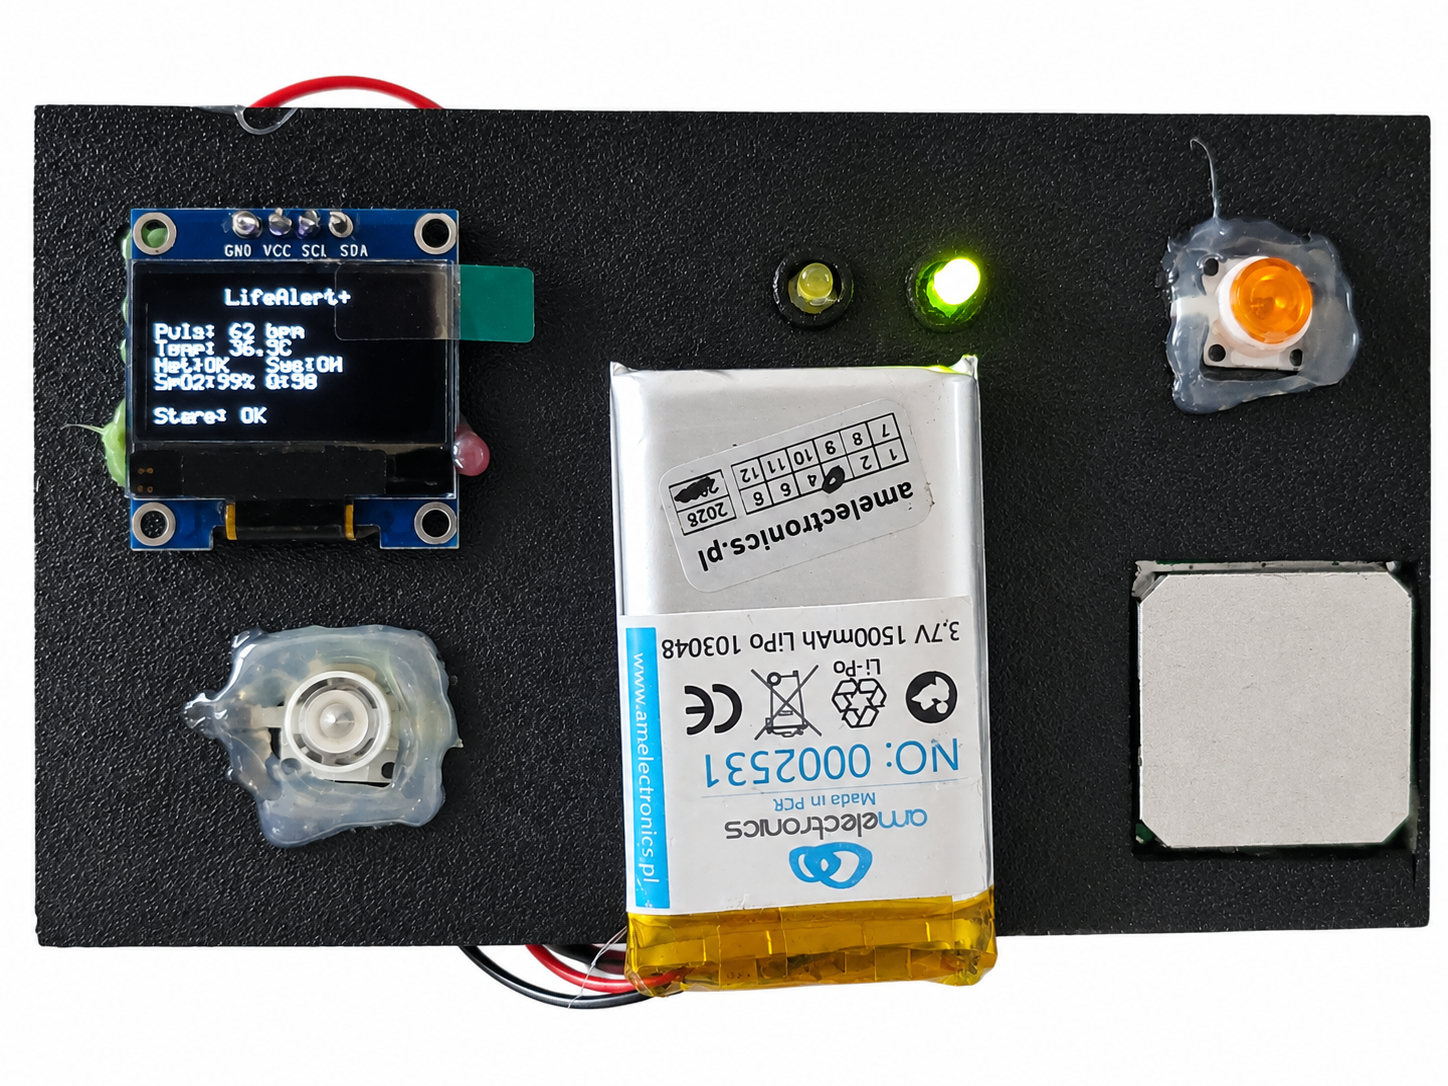
\includegraphics[width=0.72\textwidth]{figuri/interfata_dispozitiv.png}
\caption{Interfața dispozitivului portabil LifeAlertPlus: ecranul OLED afișând parametrii vitali și starea sistemului, împreună cu LED-urile de stare și butoanele de interacțiune.}
\label{fig:dispozitiv}
\end{figure}

\subsection{Prelucrarea datelor și inteligență artificială}

Datele brute furnizate de senzorii biomedicali nu pot fi utilizate direct pentru a decide dacă starea pacientului este una normală sau una care necesită intervenție. Valorile individuale, precum o frecvență cardiacă de 105 bpm sau o temperatură de 37,8\textdegree C, sunt ambigue atunci când sunt interpretate izolat: ele pot indica fie o stare patologică, fie o reacție fiziologică firească la efort, stres sau temperatura ambientală. Din acest motiv, transformarea datelor în informație utilă din punct de vedere clinic presupune o etapă de prelucrare și o etapă de interpretare, în care intervine inteligența artificială.

În sistemul dezvoltat, prelucrarea datelor este organizată pe două niveluri. Primul nivel, realizat local pe microcontroller, cuprinde filtrarea valorilor evident eronate (citiri în afara intervalelor fizic posibile, generate de contactul imperfect al senzorului cu pielea) și calculul unor mărimi derivate, precum magnitudinea vectorului de accelerație, obținută din componentele pe cele trei axe. Al doilea nivel, realizat pe server, cuprinde analiza propriu-zisă a stării de sănătate, prin combinarea unui model de învățare automată cu un set de reguli medicale deterministe.

\subsubsection{Învățarea automată și problema de clasificare}

Învățarea automată (machine learning) este subdomeniul inteligenței artificiale care studiază algoritmii capabili să își îmbunătățească performanța pe baza datelor, fără a fi programați explicit pentru fiecare situație posibilă. În cazul de față, evaluarea stării pacientului a fost formulată ca o problemă de \textbf{clasificare supervizată}: pornind de la un set de parametri vitali, modelul trebuie să atribuie pacientului una dintre trei clase, anume \texttt{NORMAL}, \texttt{ALERT} sau \texttt{CRITICAL}. Clasificarea supervizată presupune existența unui set de date de antrenare în care fiecare exemplu este însoțit de eticheta corectă, modelul deducând din aceste exemple o funcție de decizie care poate fi aplicată ulterior unor date noi.

Algoritmul utilizat este \textbf{Random Forest}, un model de tip ansamblu (ensemble) format dintr-o mulțime de arbori de decizie antrenați independent pe subseturi aleatorii ale datelor. Predicția finală rezultă din agregarea voturilor tuturor arborilor, ceea ce reduce semnificativ riscul de supraînvățare (overfitting) caracteristic unui arbore de decizie individual. Random Forest a fost preferat datorită robusteții în raport cu zgomotul din date, a capacității de a estima importanța fiecărui parametru de intrare și a faptului că nu necesită un volum de date la fel de mare ca rețelele neuronale, un avantaj practic important într-un domeniu în care datele medicale reale etichetate sunt greu de obținut. Modelul a fost configurat cu 150 de arbori, o adâncime maximă de 10 niveluri și ponderarea claselor, pentru a compensa distribuția lor inegală.

\subsubsection{Datele de antrenare și pregătirea lor}

Întrucât colectarea unui volum suficient de date medicale reale, etichetate, ridică probleme practice și de confidențialitate, modelul a fost antrenat pe un set de date sintetice, generat pornind de la trei surse publice recunoscute: setul de date BIDMC pentru frecvența cardiacă și saturația oxigenului, un set de date de termometrie pentru temperatura corporală și un set de date provenit de la senzori MPU6050 pentru parametrii de mișcare. Peste valorile extrase din aceste surse a fost adăugat un zgomot gaussian controlat, pentru a obține o variabilitate realistă, și au fost generate suplimentar exemple corespunzătoare stărilor \texttt{ALERT} și \texttt{CRITICAL}, mai rare în datele reale, astfel încât modelul să poată învăța corect și situațiile critice.

Înainte de antrenare, datele au fost supuse unor operații standard de preprocesare. Parametrii proveniți de la accelerometru și giroscop au fost normalizați prin metoda Min-Max, care aduce toate valorile în intervalul $[0, 1]$, împiedicând ca mărimile cu domeniu numeric larg să domine procesul de învățare. Etichetele textuale ale claselor au fost convertite în valori numerice prin codificare (label encoding), iar saturației oxigenului i s-a atribuit o pondere suplimentară, fiind cel mai relevant indicator clinic dintre parametrii monitorizați.

\subsubsection{Sistemul hibrid de decizie}

O caracteristică importantă a soluției este faptul că decizia finală nu este lăsată exclusiv în seama modelului de învățare automată. Predicția acestuia este combinată cu un set de \textbf{reguli medicale deterministe}, derivate din praguri clinice consacrate. Motivul acestei abordări hibride este unul de siguranță: un model de învățare automată, oricât de bine antrenat, poate produce predicții eronate în cazuri rare sau atipice, în timp ce o regulă medicală absolută (de exemplu, o saturație a oxigenului sub un prag critic clasificată automat ca stare \texttt{CRITICAL}) garantează că situațiile fără echivoc sunt tratate corect indiferent de comportamentul modelului. Astfel, modelul AI aduce capacitatea de a recunoaște tipare complexe și corelații subtile între parametri, iar regulile medicale aduc garanții de corectitudine și explicabilitate.

În plus față de starea discretă (NORMAL/ALERT/CRITICAL), sistemul calculează un \textbf{health score}, un indice sintetic cu valori între 0 și 100 care exprimă numeric gradul de risc al pacientului la un moment dat. Spre deosebire de starea discretă, health score-ul oferă o măsură continuă, care permite urmărirea tendințelor (o stare care se degradează lent, dar constant) și declanșarea graduală a alertelor. Logica de calcul a acestui indice, precum și modul în care ține cont de pragurile personalizate ale fiecărui pacient și de afecțiunile preexistente ale acestuia, sunt detaliate în capitolul de proiectare a sistemului. Schema mecanismului hibrid de decizie este prezentată în figura~\ref{fig:hibrid-ai}.

\begin{figure}[H]
\centering
\resizebox{\textwidth}{!}{%
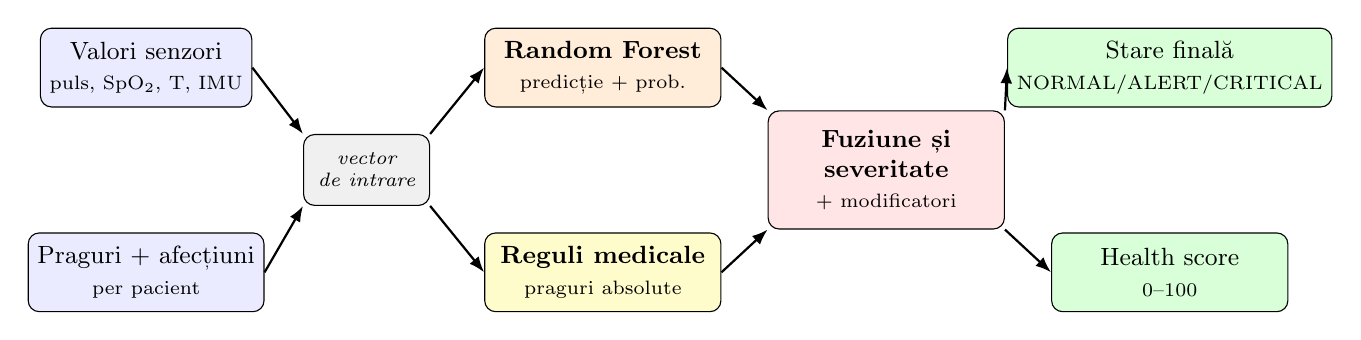
\begin{tikzpicture}[
    every node/.style={font=\small},
    input/.style={rectangle, rounded corners, draw, minimum width=2.6cm, minimum height=1.0cm, align=center, fill=blue!8},
    proc/.style={rectangle, rounded corners, draw, minimum width=3.0cm, minimum height=1.0cm, align=center, fill=orange!15},
    rules/.style={rectangle, rounded corners, draw, minimum width=3.0cm, minimum height=1.0cm, align=center, fill=yellow!20},
    fuz/.style={rectangle, rounded corners, draw, minimum width=3.0cm, minimum height=1.5cm, align=center, fill=red!10},
    outp/.style={rectangle, rounded corners, draw, minimum width=3.0cm, minimum height=1.0cm, align=center, fill=green!15},
    merger/.style={rectangle, rounded corners, draw, fill=gray!12, font=\scriptsize\itshape, align=center, inner sep=4pt, minimum height=0.9cm, minimum width=1.6cm},
    arrow/.style={-{Latex[length=2mm]}, thick}]

  \node[input] (sens) at (-6.4, 1.3) {Valori senzori\\\scriptsize puls, \spo, T, IMU};
  \node[input] (prag) at (-6.4,-1.3) {Praguri + afecțiuni\\\scriptsize per pacient};

  \node[merger] (m1) at (-3.6, 0) {vector\\de intrare};

  \node[proc]  (rf) at (-0.6, 1.3) {\textbf{Random Forest}\\\scriptsize predicție + prob.};
  \node[rules] (rg) at (-0.6,-1.3) {\textbf{Reguli medicale}\\\scriptsize praguri absolute};

  \node[fuz] (fz) at ( 3.0, 0) {\textbf{Fuziune și}\\\textbf{severitate}\\\scriptsize + modificatori};

  \node[outp] (stare) at ( 6.6, 1.3) {Stare finală\\\scriptsize NORMAL/ALERT/CRITICAL};
  \node[outp] (score) at ( 6.6,-1.3) {Health score\\\scriptsize 0--100};

  \draw[arrow] (sens.east) -- (m1.north west);
  \draw[arrow] (prag.east) -- (m1.south west);
  \draw[arrow] (m1.north east) -- (rf.west);
  \draw[arrow] (m1.south east) -- (rg.west);
  \draw[arrow] (rf.east) -- (fz.north west);
  \draw[arrow] (rg.east) -- (fz.south west);
  \draw[arrow] (fz.north east) -- (stare.west);
  \draw[arrow] (fz.south east) -- (score.west);
\end{tikzpicture}}
\caption{Mecanismul hibrid de decizie: senzorii și pragurile personalizate formează un vector de intrare comun, evaluat în paralel de modelul Random Forest și de setul de reguli medicale; predicțiile sunt combinate în stratul de fuziune, care produce simultan starea discretă și health score-ul.}
\label{fig:hibrid-ai}
\end{figure}

\subsubsection{Explicabilitatea și evaluarea modelului}

Într-un domeniu cu implicații medicale, un model care produce predicții corecte, dar de neînțeles, este insuficient: este necesar ca decizia să poată fi explicată. Din acest motiv, modelul a fost analizat folosind metoda \textbf{SHAP (SHapley Additive exPlanations)}, o tehnică ce cuantifică contribuția fiecărui parametru de intrare la o predicție individuală. Analiza SHAP a confirmat că saturația oxigenului, frecvența cardiacă și temperatura corporală sunt factorii dominanți în decizia modelului, în concordanță cu criteriile clinice de triaj.

Performanța modelului a fost estimată prin \textbf{validare încrucișată stratificată în 5 falduri} (stratified 5-fold cross-validation), o metodă prin care setul de date este împărțit repetat în subseturi de antrenare și testare, păstrând în fiecare fald aceeași distribuție a claselor. Această abordare oferă o estimare mai realistă a capacității de generalizare decât o singură împărțire antrenare/testare și permite, totodată, verificarea absenței supraînvățării prin compararea performanței pe datele de antrenare cu cea pe datele de testare. Au fost urmărite metrici precum acuratețea, scorul F1 și aria de sub curba ROC.

\subsubsection{Clasificarea activității și arhitectura de tip microserviciu}

Pe lângă evaluarea stării de sănătate, datele de mișcare furnizate de senzorul MPU6050 sunt prelucrate \textbf{pe dispozitiv} pentru a clasifica activitatea purtătorului ca \texttt{moving} sau \texttt{stationary}, și pentru a contribui la detectarea căderilor. Eticheta de activitate este derivată din acumularea abaterii magnitudinii acceleraţiei faţă de gravitaţie ($|\vec{a}| - 1\,g$) peste fereastra de ~5\,s între două POST-uri: media şi maximul abaterii peste această fereastră sunt comparate cu praguri empirice (0,05\,g pentru media de mişcare susţinută, 0,20\,g pentru un vârf izolat), iar eticheta rezultată este inclusă direct în payload-ul JSON trimis backend-ului. Această clasificare reutilizează exact aceleaşi sample-uri pe care fall-detector-ul le citește la 50\,Hz, fără overhead suplimentar. Pe baza acestei etichete, persistată pentru fiecare măsurătoare, backend-ul agregă \textbf{profilul de activitate zilnică} (rata de mişcare şi probabilitatea de somn per oră, pe o fereastră de 7 zile) şi detectează două tipuri de anomalii comportamentale: \textit{inactivitate prelungită} (peste 15 minute fără mişcare într-o oră în care pacientul e de obicei activ) şi \textit{activitate nocturnă} (mişcare detectată într-o oră în care pacientul doarme de obicei).

Din punct de vedere arhitectural, componenta de inteligență artificială propriu-zisă (clasificarea stării vitale în NORMAL/ALERT/CRITICAL şi calculul health score-ului) este implementată ca un \textbf{microserviciu} independent, scris în limbajul Python și expus printr-o interfață REST. Această separare a fost aleasă deliberat: ecosistemul Python oferă cele mai mature biblioteci de învățare automată, iar izolarea modulului AI într-un serviciu propriu permite actualizarea, înlocuirea sau scalarea modelului fără a afecta restul aplicației. Backend-ul aplicației comunică cu microserviciul AI prin cereri HTTP, transmițând valorile senzorilor și primind în răspuns starea prezisă, health score-ul și o explicație textuală a deciziei.

\subsection{Sisteme de alertare}

Un sistem de alertare reprezintă ansamblul de mecanisme prin care un sistem informatic semnalează automat apariția unei situații care necesită atenție. În contextul monitorizării medicale, sistemul de alertare este componenta care transformă o anomalie detectată într-o acțiune concretă: informarea unei persoane capabile să intervină. Funcționarea sa presupune trei etape succesive, anume detectarea evenimentului, decizia de a alerta și livrarea efectivă a notificării.

\subsubsection{Fiabilitate și problema alertelor false}

Cerința fundamentală a unui sistem de alertare medicală este fiabilitatea, înțeleasă în dublu sens: sistemul trebuie să semnaleze toate situațiile reale de risc (sensibilitate ridicată), dar trebuie, în același timp, să evite alarmele nejustificate (specificitate ridicată). Un sistem care generează frecvent alerte false produce fenomenul cunoscut sub numele de \textit{alert fatigue}, adică obișnuirea destinatarului cu notificările, urmată de ignorarea acestora, inclusiv a celor reale. Pentru o aplicație destinată siguranței persoanelor vârstnice, acest efect ar anula însuși scopul sistemului.

Din acest motiv, sistemele de alertare moderne includ mai multe mecanisme de reducere a alertelor false. \textbf{Pragul de persistență} impune ca o situație anormală să se mențină o durată minimă de timp înainte de a declanșa o notificare, eliminând astfel valorile tranzitorii cauzate de un contact imperfect al senzorului. Mecanismul de \textbf{cooldown} (perioadă de inhibare) împiedică transmiterea repetată a aceleiași alerte într-un interval scurt, evitând inundarea destinatarului cu mesaje. \textbf{Escaladarea} presupune trecerea succesivă la canale de comunicație mai insistente atunci când o alertă nu este confirmată; de exemplu, o notificare push poate fi urmată de un SMS dacă situația persistă.

\subsubsection{Alertarea multi-canal}

Niciun canal de comunicație nu este, singur, suficient de fiabil pentru un scenariu medical. Din acest motiv, soluția propusă utilizează trei canale complementare, fiecare cu caracteristici proprii.

\textbf{SMS}: mesajele text reprezintă canalul cu cea mai mare acoperire, întrucât nu necesită ca destinatarul să dețină un smartphone, o aplicație instalată sau o conexiune la internet. SMS-ul este deosebit de potrivit pentru notificarea aparținătorilor în orice condiții. Livrarea SMS-urilor se realizează prin intermediul unei platforme de comunicație în cloud (CPaaS, adică Communication Platform as a Service), care expune o interfață de programare prin care aplicația poate trimite mesaje fără a gestiona direct infrastructura de telefonie.

\textbf{Email}: poșta electronică este potrivită pentru notificări mai puțin urgente și pentru transmiterea de conținut bogat: rapoarte, grafice, atașamente. Spre deosebire de SMS, livrarea email-ului nu este garantată în timp real și poate fi întârziată sau filtrată ca spam, motiv pentru care este utilizată ca un canal complementar, nu ca singura cale de alertare.

\textbf{Notificările push}: acestea sunt mesaje livrate instantaneu în interfața aplicației web, atâta vreme cât aceasta este deschisă. Notificările push oferă cea mai mică latență dintre toate canalele și sunt ideale pentru actualizarea în timp real a tabloului de bord al aparținătorului. Ele depind însă de existența unei conexiuni active, motiv pentru care sunt dublate de SMS în situațiile critice.

Combinarea celor trei canale asigură redundanță: dacă un canal eșuează sau nu este observat, un altul preia rolul de informare, crescând probabilitatea ca aparținătorul să fie alertat la timp. Fluxul comparativ al celor trei canale este sintetizat în figura~\ref{fig:multi-canal}.

\begin{figure}[H]
\centering
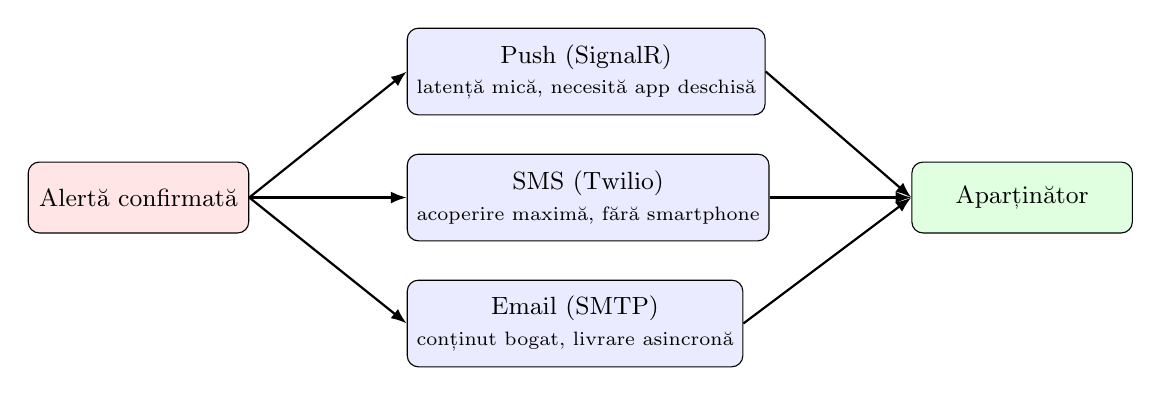
\begin{tikzpicture}[node distance=0.7cm and 1.6cm,
    every node/.style={font=\small},
    src/.style={rectangle, rounded corners, draw, minimum width=2.8cm, minimum height=0.9cm, align=center, fill=red!10},
    chan/.style={rectangle, rounded corners, draw, minimum width=3.0cm, minimum height=1.1cm, align=center, fill=blue!8},
    dest/.style={rectangle, rounded corners, draw, minimum width=2.8cm, minimum height=0.9cm, align=center, fill=green!12},
    arrow/.style={-{Latex[length=2mm]}, thick}]

  \node[src] (alerta) {Alertă confirmată};

  \node[chan, right=2.0cm of alerta, yshift=1.6cm] (push) {Push (SignalR)\\\scriptsize latență mică, necesită app deschisă};
  \node[chan, right=2.0cm of alerta] (sms) {SMS (Twilio)\\\scriptsize acoperire maximă, fără smartphone};
  \node[chan, right=2.0cm of alerta, yshift=-1.6cm] (mail) {Email (SMTP)\\\scriptsize conținut bogat, livrare asincronă};

  \node[dest, right=1.8cm of sms] (apar) {Aparținător};

  \draw[arrow] (alerta.east) -- (push.west);
  \draw[arrow] (alerta.east) -- (sms.west);
  \draw[arrow] (alerta.east) -- (mail.west);
  \draw[arrow] (push.east) -- (apar.west);
  \draw[arrow] (sms.east) -- (apar.west);
  \draw[arrow] (mail.east) -- (apar.west);
\end{tikzpicture}
\caption{Livrarea alertei prin trei canale complementare asigură redundanța mecanismului de notificare.}
\label{fig:multi-canal}
\end{figure}

\subsection{Tehnologii utilizate (backend, frontend, Docker etc.)}

Realizarea unui sistem IoT funcțional, dincolo de componenta hardware, presupune integrarea unui set coerent de tehnologii software. Această secțiune prezintă pe scurt tehnologiile pe care se sprijină aplicația, grupate pe niveluri arhitecturale.

\subsubsection{Backend-ul aplicației}

Backend-ul reprezintă nivelul de procesare al sistemului și a fost dezvoltat folosind \textbf{ASP.NET Core}, un framework open-source și cross-platform dezvoltat de Microsoft pentru construirea de aplicații web și interfețe de programare, utilizând limbajul C\#. Backend-ul expune un \textbf{API REST}, un stil arhitectural bazat pe protocolul HTTP, în care resursele sunt accesate prin verbe standard (GET, POST, PUT, DELETE), iar datele sunt schimbate în format JSON. Prin acest API comunică atât dispozitivele IoT, care transmit măsurătorile, cât și aplicația web, care le consultă.

Codul backend-ului este organizat conform principiilor unei \textbf{arhitecturi stratificate (clean architecture)}, separat în mai multe straturi cu responsabilități distincte: stratul de domeniu, care conține entitățile fundamentale; stratul de aplicație, care conține logica de business; stratul de infrastructură, responsabil cu accesul la date și cu serviciile externe; și stratul de prezentare a API-ului, care conține controlerele. Această separare facilitează testarea, întreținerea și extinderea ulterioară a sistemului.

Persistența datelor este asigurată de o bază de date relațională \textbf{SQLite}, un sistem de baze de date încorporat, care stochează întreaga bază într-un singur fișier și nu necesită un server dedicat. Accesul la baza de date se realizează prin intermediul unui ORM (Object-Relational Mapper), anume \textbf{Entity Framework Core}, care mapează automat clasele din cod pe tabelele bazei de date și permite formularea interogărilor direct în limbajul C\#.

\subsubsection{Securitatea}

Întrucât sistemul gestionează date medicale, securitatea reprezintă o cerință esențială. Autentificarea utilizatorilor se bazează pe \textbf{JWT (JSON Web Token)}, un mecanism de autentificare fără stare în care, după autentificare, serverul emite un token semnat criptografic ce conține informații despre utilizator și care este prezentat la fiecare cerere ulterioară. Aplicația permite, de asemenea, autentificarea prin \textbf{OAuth 2.0} folosind un cont Google, un protocol standard de autorizare delegată care elimină necesitatea gestionării unei parole suplimentare. Parolele utilizatorilor care aleg înregistrarea clasică sunt stocate sub formă de hash generat cu algoritmul \textbf{BCrypt}, conceput special pentru a fi lent și rezistent la atacuri de tip forță brută.

\subsubsection{Comunicarea în timp real}

Pentru actualizarea instantanee a interfeței și pentru livrarea notificărilor push, sistemul folosește \textbf{SignalR}, o bibliotecă care permite comunicarea bidirecțională în timp real între server și client. SignalR abstractizează protocolul WebSocket, menținând o conexiune permanentă prin care serverul poate transmite mesaje către client fără ca acesta să le ceară explicit.

\subsubsection{Frontend-ul aplicației}

Interfața web a fost dezvoltată folosind \textbf{Blazor WebAssembly}, un framework care permite scrierea aplicațiilor web interactive în limbajul C\#, fără a fi necesar JavaScript pentru logica aplicației. Codul C\# este compilat în \textbf{WebAssembly}, un format binar de instrucțiuni care rulează direct în browser, la o viteză apropiată de cea nativă. Aplicația este o \textbf{SPA (Single-Page Application)}, adică o aplicație web care se încarcă o singură dată și care actualizează dinamic conținutul, fără reîncărcarea completă a paginii.

Aplicația este, în plus, o \textbf{PWA (Progressive Web Application)}: include un service worker care permite funcționarea parțială în lipsa conexiunii la internet, un fișier manifest care permite instalarea aplicației pe dispozitiv ca o aplicație nativă și o pagină dedicată pentru modul offline.

\subsubsection{Containerizarea și implementarea}

Pentru asigurarea consistenței între mediul de dezvoltare și cel de producție, componentele aplicației sunt împachetate folosind \textbf{Docker}, o tehnologie de containerizare care încapsulează o aplicație împreună cu toate dependențele sale într-o imagine portabilă. Cele trei componente principale ale sistemului, anume microserviciul AI, backend-ul și frontend-ul, sunt orchestrate prin \textbf{Docker Compose}, un instrument care permite definirea și pornirea coordonată a mai multor containere. Servirea fișierelor statice ale interfeței web este realizată printr-un server \textbf{nginx}.

Procesul de construire, testare și publicare a aplicației este automatizat printr-un flux de \textbf{integrare și livrare continuă (CI/CD)} configurat cu GitHub Actions, iar sistemul este deployat pe infrastructura cloud \textbf{Microsoft Azure}, asigurând disponibilitatea și accesul de la distanță.

\newpage
\section{Analiza soluțiilor existente}

\subsection{Prezentarea soluțiilor actuale}

Piața dispozitivelor de monitorizare medicală portabilă a cunoscut o expansiune semnificativă în ultimul deceniu, atât din perspectiva soluțiilor comerciale de masă, cât și a sistemelor dedicate mediului clinic sau îngrijirii persoanelor vârstnice. În cele ce urmează sunt prezentate cele mai relevante categorii de soluții existente, analizate din perspectiva funcționalității, a publicului țintă și a tehnologiilor utilizate.

\subsubsection{Fitbit Sense 2 / Google Pixel Watch}

Fitbit, achiziționat de Google în 2021, reprezintă unul dintre cele mai cunoscute ecosisteme de monitorizare a sănătății destinate publicului larg. Dispozitivele din gama Sense monitorizează frecvența cardiacă, \spo, temperatura pielii, nivelul de stres prin electrodermal activity (EDA) și calitatea somnului. Datele sunt sincronizate prin BLE cu aplicația mobilă Fitbit, disponibilă pe Android și iOS, și stocate în cloud-ul Google.

Deși ecosistemul Fitbit este matur și bine documentat, el este proiectat pentru utilizatori activi, orientați spre fitness și auto-monitorizare. Interfața aplicației presupune un nivel de familiarizare digitală incompatibil cu profilul persoanelor vârstnice, iar sistemul de alertare este limitat la notificări generale, fără posibilitatea configurării unor praguri personalizate sau a notificării unui aparținător desemnat.

\subsubsection{Apple Watch (Series 9 / Ultra 2)}

Apple Watch reprezintă cel mai avansat dispozitiv portabil de monitorizare a sănătății disponibil comercial. Seria 9 include senzori pentru ECG, frecvență cardiacă, \spo, temperatură și detecție a căderilor, aceasta din urmă fiind direct relevantă pentru scenariul persoanelor vârstnice. Funcția Emergency SOS permite contactarea serviciilor de urgență automat după detectarea unei căderi, dacă utilizatorul nu răspunde în intervalul de timp configurat.

Cu toate acestea, Apple Watch necesită un iPhone asociat pentru configurare și funcționare completă, ceea ce presupune că pacientul trebuie să dețină și să opereze un smartphone Apple, o cerință nerealistă pentru majoritatea persoanelor vârstnice din România. Costul ridicat al ecosistemului (dispozitiv + abonament iCloud) reprezintă o barieră suplimentară. Mai mult, platforma este închisă, nepermițând integrarea cu sisteme externe de monitorizare sau exportul structurat al datelor către un medic sau aparținător prin canale personalizate.

\subsubsection{Philips Lifeline / Medical Guardian}

Philips Lifeline și Medical Guardian reprezintă o categorie distinctă de dispozitive, anume sistemele de alertă personală medicală (PERS, adică Personal Emergency Response Systems), dedicate exclusiv persoanelor vârstnice sau cu mobilitate redusă. Acestea iau forma unor butoane de panică purtate ca pandantiv sau brățară, conectate la o centrală care permite contactarea unui operator uman sau a serviciilor de urgență.

Avantajul principal al acestor sisteme este simplitatea extremă din perspectiva utilizatorului, anume un singur buton fizic. Dezavantajul major este că nu realizează monitorizare continuă a parametrilor vitali. Sistemul reacționează exclusiv la inițiativa pacientului, ceea ce îl face ineficient în scenarii precum pierderea conștienței, căderea cu imobilizare sau degradarea lentă a stării de sănătate, când pacientul este incapabil să apese butonul.

\subsubsection{Withings ScanWatch}

Withings ScanWatch este un ceas inteligent cu design clasic, care monitorizează frecvența cardiacă, \spo, respirația în somn și activitatea fizică. Spre deosebire de Fitbit sau Apple Watch, ScanWatch are un design discret, similar unui ceas tradițional, ceea ce îl face mai acceptabil estetic pentru utilizatorii vârstnici. Autonomia bateriei de până la 30 de zile reprezintă un avantaj semnificativ față de concurență.

Totuși, și Withings ScanWatch este orientat spre auto-monitorizare, fără un sistem dedicat de alertare a aparținătorilor și fără posibilitatea configurării unor praguri personalizate de alertă. Exportul datelor se face prin aplicația Health Mate, care nu oferă funcționalitate de tip dashboard pentru o persoană terță (aparținător).

\subsubsection{Soluții academice și de cercetare}

Literatura de specialitate propune numeroase sisteme IoT de monitorizare medicală dezvoltate în context academic, bazate frecvent pe platforme Arduino sau ESP32, senzori MAX30100/MAX30102 și protocoale MQTT pentru transmisia datelor. Aceste sisteme demonstrează viabilitatea tehnică a abordării, însă rămân în stadiul de prototip de laborator, fără interfețe utilizator complete, fără mecanisme de alertare multi-canal și fără considerarea aspectelor practice legate de autonomia bateriei, rezistența mecanică sau ușurința de utilizare pentru persoane fără competențe tehnice.

\subsection{Limitări identificate}

Analiza soluțiilor prezentate în secțiunea anterioară relevă o serie de limitări comune, grupate în câteva categorii principale.

\subsubsection{Inadecvarea pentru utilizatorii vârstnici}

Majoritatea soluțiilor comerciale sunt proiectate pentru utilizatori tineri sau de vârstă medie, cu competențe digitale solide. Interfețele complexe, necesitatea unui smartphone asociat și procesele de configurare multi-pas reprezintă bariere reale pentru persoanele vârstnice. Sistemele PERS (Philips Lifeline, Medical Guardian) rezolvă parțial această problemă prin simplitate, dar sacrifică complet monitorizarea continuă.

\subsubsection{Lipsa monitorizării continue și a alertării inteligente}

Dispozitivele comerciale de tip smartwatch alertează utilizatorul însuși, nu un aparținător desemnat. Scenariul critic, în care pacientul este incapabil să reacționeze, iar aparținătorul rămâne neinformat, nu este acoperit adecvat de niciuna dintre soluțiile analizate. Sistemele PERS depind exclusiv de inițiativa pacientului, iar smartwatch-urile nu oferă un mecanism fiabil de escaladare a alertelor către persoane terțe prin canale multiple (SMS, email, push).

\subsubsection{Platforme închise și lipsa personalizării}

Soluțiile comerciale funcționează în ecosisteme închise care nu permit integrarea cu sisteme externe, configurarea pragurilor de alertă în funcție de profilul medical individual sau exportul structurat al datelor. Un medic nu poate accesa direct datele unui pacient care folosește Fitbit sau Apple Watch fără ca pacientul să realizeze manual operațiuni de export.

\subsubsection{Costul și dependența de abonamente}

Atât Apple Watch, cât și sistemele PERS implică costuri recurente, precum abonamente cloud sau taxe lunare pentru servicii de monitorizare umană, care pot fi prohibitive pe termen lung, în special pentru persoane cu venituri fixe reduse, categorie frecvent suprapusă cu cea a vârstnicilor.

\subsubsection{Limitări ale soluțiilor academice}

Prototipurile academice demonstrează conceptul tehnic, dar nu adresează aspecte esențiale pentru un sistem funcțional real: interfață utilizator completă, securitatea datelor medicale, mecanisme de recuperare la pierderea conexiunii, autonomia bateriei în condiții reale de utilizare sau scalabilitatea la număr mare de utilizatori.

Tabelul~\ref{tab:comparatie} sintetizează comparativ limitările identificate.

\begin{table}[H]
\centering
\small
\renewcommand{\arraystretch}{1.3}
\begin{tabular}{|>{\raggedright\arraybackslash}p{3.0cm}|p{1.7cm}|p{1.7cm}|p{1.9cm}|p{1.5cm}|p{1.9cm}|}
\hline
\textbf{Criteriu} & \textbf{FitBit/ Google} & \textbf{Apple Watch} & \textbf{Philips Lifeline} & \textbf{Withings} & \textbf{Soluții academice}\\
\hline
Potrivit pentru vârstnici & Parțial & Nu & Da & Parțial & Nu\\
\hline
Monitorizare continuă vitale & Da & Da & Nu & Da & Da\\
\hline
Alertare aparținător multi-canal & Nu & Nu & Parțial & Nu & Nu\\
\hline
Praguri personalizabile & Nu & Nu & Nu & Nu & Parțial\\
\hline
Export date structurat & Limitat & Limitat & Nu & Limitat & Parțial\\
\hline
Fără abonament obligatoriu & Nu & Nu & Nu & Nu & Da\\
\hline
Stocare locală la pierdere semnal & Nu & Nu & Nu & Nu & Nu\\
\hline
Detecție căderi & Nu & Da & Nu & Nu & Nu\\
\hline
Healthscore integrat & Nu & Nu & Nu & Nu & Nu\\
\hline
\end{tabular}
\caption{Comparație între soluțiile existente și limitările identificate.}
\label{tab:comparatie}
\end{table}

\subsection{Poziționarea soluției propuse}

Soluția dezvoltată în cadrul acestei lucrări se poziționează într-un spațiu neacoperit adecvat de produsele existente: un sistem de monitorizare continuă a parametrilor vitali, dedicat persoanelor vârstnice, cu alertare automată multi-canal a aparținătorilor și configurare tehnică minimă din partea pacientului.

Față de soluțiile comerciale de tip smartwatch, sistemul propus oferă:

\begin{itemize}[leftmargin=1.5em]
\item \textbf{Alertare activă a aparținătorului} prin SMS, email și notificări push, fără a depinde de inițiativa pacientului;
\item \textbf{Praguri de alertă personalizabile} per pacient, configurabile de aparținător din aplicația web;
\item \textbf{Health score}, un indice sintetic al stării de sănătate bazat pe corelarea mai multor parametri vitali simultan, absent din oricare dintre soluțiile analizate;
\item \textbf{Stocare locală a datelor} la pierderea conectivității, cu sincronizare automată la revenirea semnalului;
\item \textbf{Export structurat} al datelor direct către medicul curant, prin email, dintr-un interval selectabil.
\end{itemize}

Față de sistemele PERS (butoane de panică), soluția propusă adaugă monitorizarea continuă și detecția automată a situațiilor critice, eliminând dependența de capacitatea pacientului de a apăsa un buton în momentul critic.

Față de prototipurile academice, sistemul propus depășește stadiul de demonstrație tehnică prin includerea unei interfețe web complete, a unui sistem de autentificare securizat, a unui mecanism de notificări funcțional și a unei arhitecturi deployate pe infrastructură cloud reală.

Această poziționare confirmă relevanța și originalitatea soluției propuse, care nu încearcă să concureze frontal cu ecosistemele comerciale mature, ci adresează un segment specific și insuficient acoperit: monitorizarea continuă, automată și inteligentă a persoanelor vârstnice, cu implicarea activă a aparținătorului prin tehnologii accesibile și fără costuri recurente semnificative.

\newpage
\section{Proiectarea sistemului}

Acest capitol descrie deciziile de proiectare luate înaintea implementării propriu-zise. Sunt prezentate, pe rând, arhitectura de ansamblu a sistemului, componentele care îl alcătuiesc și rolul fiecăreia, structura bazei de date și, în final, fluxurile prin care datele circulă prin sistem, de la achiziția lor pe dispozitiv până la declanșarea unei alerte. Tot aici este detaliată logica mecanismului health score, anunțată în subcapitolul 2.3.

\subsection{Arhitectura generală}

Sistemul LifeAlertPlus respectă modelul arhitectural pe trei niveluri specific aplicațiilor IoT, prezentat în subcapitolul 2.1. Fiecărui nivel teoretic îi corespunde o componentă concretă: nivelului de percepție îi corespunde dispozitivul portabil bazat pe microcontrollerul ESP32-C3 Mini; nivelului de rețea îi corespunde comunicația WiFi; iar nivelului de aplicație îi corespund backend-ul, microserviciul de inteligență artificială, baza de date și aplicația web, toate găzduite pe infrastructură cloud.

\subsubsection{Separarea în straturi a aplicației software}

Partea software a sistemului a fost proiectată conform principiilor unei arhitecturi stratificate (clean architecture), în care responsabilitățile sunt împărțite între mai multe straturi cu dependențe orientate într-un singur sens, dinspre exterior spre interior. Concret, soluția este organizată în următoarele proiecte:

\begin{itemize}[leftmargin=1.5em]
\item \textbf{Domain}: conține entitățile fundamentale ale sistemului (utilizator, persoană monitorizată, măsurătoare etc.) și interfețele depozitelor de date. Acest strat nu depinde de niciun alt strat și nu cunoaște detalii de implementare.
\item \textbf{Application}: conține logica de business, organizată în servicii, și interfețele acestora. Depinde exclusiv de stratul Domain.
\item \textbf{Infrastructure}: conține implementările concrete, anume contextul bazei de date și depozitele realizate cu Entity Framework Core, precum și integrările cu servicii externe. Depinde de Application și Domain.
\item \textbf{API}: stratul de prezentare al backend-ului, care expune controlerele REST, serviciile de fundal și configurarea aplicației.
\item \textbf{Client}: aplicația web Blazor WebAssembly, executată în browserul utilizatorului.
\item \textbf{Shared}: conține obiectele de transfer de date (DTO) folosite în comun de backend și de client, asigurând un contract unic de comunicare.
\end{itemize}

Avantajul acestei separări este că logica de business rămâne independentă de tehnologiile concrete: baza de date SQLite, de exemplu, ar putea fi înlocuită fără a modifica straturile Domain și Application. Totodată, structura facilitează testarea izolată a fiecărui strat și întreținerea pe termen lung.

\subsubsection{Microserviciul de inteligență artificială}

Spre deosebire de celelalte componente software, scrise în C\#, componenta de inteligență artificială este un microserviciu independent, scris în Python. Această decizie de proiectare a fost luată deliberat, din două motive: ecosistemul Python oferă cele mai mature biblioteci de învățare automată, iar izolarea modelului într-un serviciu propriu permite reantrenarea sau înlocuirea acestuia fără a afecta restul aplicației. Backend-ul comunică cu microserviciul AI prin cereri HTTP, cu un timp maxim de așteptare scurt, astfel încât o eventuală indisponibilitate a serviciului AI să nu blocheze fluxul principal.

\subsubsection{Comunicarea între componente}

Componentele sistemului comunică prin trei mecanisme distincte. Dispozitivul IoT și aplicația web comunică cu backend-ul prin \textbf{API-ul REST}, peste HTTPS. Backend-ul comunică cu microserviciul AI tot prin HTTP. Pentru actualizarea instantanee a interfeței și pentru livrarea notificărilor push, backend-ul comunică cu aplicația web printr-o conexiune permanentă \textbf{WebSocket}, gestionată de biblioteca SignalR. Cele trei componente principale, adică microserviciul AI, backend-ul și frontend-ul, sunt împachetate în containere Docker și orchestrate prin Docker Compose, ceea ce asigură consistența între mediul de dezvoltare și cel de producție. Ansamblul componentelor și al legăturilor dintre ele este prezentat în figura~\ref{fig:arhitectura}.

\begin{figure}[H]
\centering
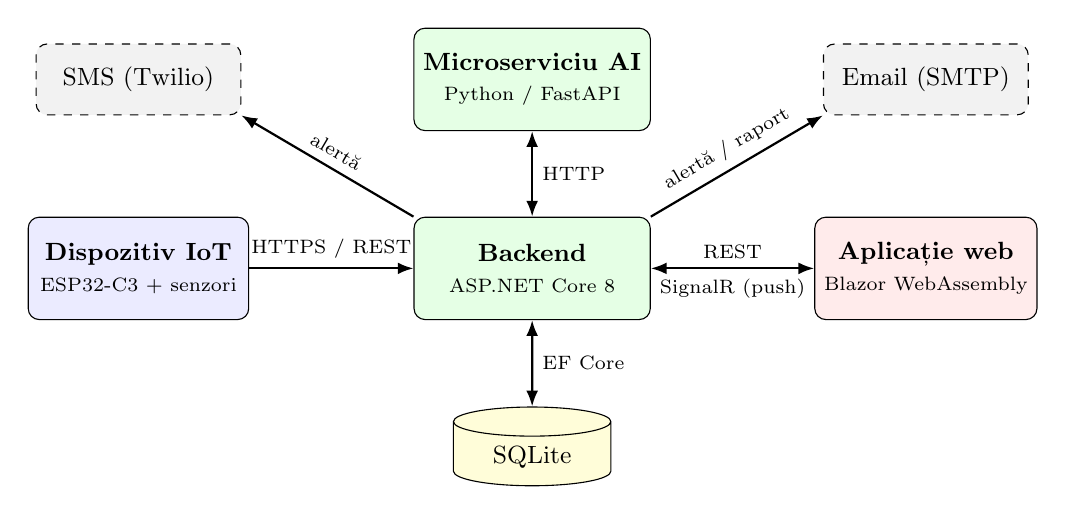
\begin{tikzpicture}[
    every node/.style={font=\small},
    dev/.style={rectangle, rounded corners, draw, minimum width=2.8cm, minimum height=1.3cm, align=center, fill=blue!8},
    srv/.style={rectangle, rounded corners, draw, minimum width=3.0cm, minimum height=1.3cm, align=center, fill=green!10},
    db/.style={cylinder, shape border rotate=90, draw, minimum width=2.0cm, minimum height=1.0cm, aspect=0.3, align=center, fill=yellow!15},
    web/.style={rectangle, rounded corners, draw, minimum width=2.8cm, minimum height=1.3cm, align=center, fill=red!8},
    ext/.style={rectangle, rounded corners, draw, dashed, minimum width=2.6cm, minimum height=0.9cm, align=center, fill=gray!10},
    arrow/.style={-{Latex[length=2mm]}, thick},
    biarrow/.style={{Latex[length=2mm]}-{Latex[length=2mm]}, thick}]

  \node[srv] (back) at (0,0) {\textbf{Backend}\\\scriptsize ASP.NET Core 8};
  \node[srv] (ai)   at (0,2.4) {\textbf{Microserviciu AI}\\\scriptsize Python / FastAPI};
  \node[db]  (sql)  at (0,-2.4) {SQLite};
  \node[dev] (esp)  at (-5.0,0) {\textbf{Dispozitiv IoT}\\\scriptsize ESP32-C3 + senzori};
  \node[web] (cli)  at (5.0,0) {\textbf{Aplicație web}\\\scriptsize Blazor WebAssembly};

  \node[ext] (twilio) at (-5.0,2.4) {SMS (Twilio)};
  \node[ext] (smtp)   at ( 5.0,2.4) {Email (SMTP)};

  \draw[arrow] (esp.east) -- node[above, font=\scriptsize]{HTTPS / REST} (back.west);
  \draw[biarrow] (back.east) -- node[above, font=\scriptsize]{REST}
                            node[below, font=\scriptsize]{SignalR (push)} (cli.west);
  \draw[biarrow] (back.north) -- node[right, font=\scriptsize]{HTTP} (ai.south);
  \draw[biarrow] (back.south) -- node[right, font=\scriptsize]{EF Core} (sql.north);
  \draw[arrow] (back.north west) -- node[above, font=\scriptsize, sloped]{alertă} (twilio.south east);
  \draw[arrow] (back.north east) -- node[above, font=\scriptsize, sloped]{alertă / raport} (smtp.south west);
\end{tikzpicture}
\caption{Arhitectura generală a sistemului LifeAlertPlus, cu backend-ul în centru și serviciile externe (Twilio, SMTP) reprezentate prin contururi punctate.}
\label{fig:arhitectura}
\end{figure}

\subsubsection{Modelul de deployment}

Cele trei componente software ale sistemului, anume microserviciul AI, backend-ul și aplicația web, sunt împachetate fiecare într-o imagine Docker proprie și pornite coordonat. Această izolare a fost o decizie de proiectare deliberată: fiecare componentă poate fi actualizată, repornită sau scalată independent de celelalte, iar mediul de execuție rămâne identic în dezvoltare și în producție. Datele persistente, adică baza de date SQLite, sunt păstrate într-un volum separat de containere, astfel încât informația să nu se piardă la reconstruirea sau actualizarea acestora.

În producție, sistemul este găzduit pe infrastructura cloud Microsoft Azure. Procesul de construire și publicare a imaginilor este automatizat printr-un flux de integrare și livrare continuă (CI/CD): la fiecare modificare a codului, componentele sunt reconstruite și, după validare, publicate automat, ceea ce reduce riscul erorilor manuale și asigură consistența între versiuni.

\subsection{Componentele sistemului}

\subsubsection{Dispozitivul portabil}

Dispozitivul portabil este construit în jurul microcontrollerului ESP32-C3 Mini și integrează senzorii descriși în subcapitolul 2.2: MAX30100 pentru puls și \spo, GY-906 MLX90614 pentru temperatură, MPU6050 pentru mișcare și NEO-6M pentru poziție. Microcontrollerul colectează periodic datele de la senzori, calculează local mărimi derivate, le afișează pe ecranul OLED și le transmite către backend. Frecvența de transmitere este configurabilă, fiind stabilită de aparținător din aplicația web. Atunci când conexiunea la internet nu este disponibilă, măsurătorile sunt stocate temporar într-o coadă locală pe dispozitiv și transmise ulterior, la revenirea conexiunii. Dispozitivul trimite periodic și un mesaj de tip \textit{heartbeat}, care raportează starea sa tehnică, anume puterea semnalului, memoria liberă, timpul de funcționare și numărul de măsurători aflate în coada de așteptare.

\subsubsection{Backend-ul}

Backend-ul reprezintă nucleul logic al sistemului. El expune API-ul REST prin care comunică dispozitivele și aplicația web, validează și autorizează cererile, persistă datele în baza de date și coordonează evaluarea stării de sănătate și declanșarea alertelor. Pe lângă controlerele care răspund cererilor, backend-ul include și servicii de fundal care rulează continuu, independent de cereri: serviciul de monitorizare a alertelor, care analizează măsurătorile primite pentru a detecta situații de risc susținute, și serviciul de raportare zilnică, care generează și trimite periodic rapoarte de sănătate.

\subsubsection{Microserviciul de inteligență artificială}

Microserviciul AI primește valorile senzorilor și pragurile personalizate ale pacientului și returnează starea de sănătate prezisă (NORMAL, ALERT sau CRITICAL), health score-ul și o explicație textuală a deciziei. Funcționarea sa internă, anume modelul Random Forest combinat cu reguli medicale deterministe, a fost descrisă în subcapitolul 2.3.

\subsubsection{Aplicația web}

Aplicația web este interfața prin care utilizatorii umani interacționează cu sistemul. Ea deservește mai multe categorii de utilizatori, cu drepturi diferite: aparținătorul, care monitorizează una sau mai multe persoane și configurează pragurile și preferințele de notificare; medicul, care primește acces la datele unui pacient prin invitație; și administratorul, care gestionează sistemul. Aplicația oferă un tablou de bord cu starea curentă a persoanei monitorizate, vizualizarea grafică a istoricului măsurătorilor, configurarea pragurilor de alertă, gestionarea notificărilor și localizarea pe hartă a pacientului în scenarii de alertă.

\subsubsection{Baza de date}

Persistența datelor este asigurată de o bază de date relațională SQLite, accesată prin ORM-ul Entity Framework Core. Baza de date stochează utilizatorii, persoanele monitorizate, istoricul măsurătorilor, notificările și datele agregate. Structura sa este detaliată în subcapitolul următor.

\subsubsection{Serviciile externe}

Sistemul integrează mai multe servicii externe: o platformă de comunicație în cloud pentru trimiterea SMS-urilor, un server SMTP pentru email, furnizorul de identitate Google pentru autentificarea prin OAuth și un serviciu de date geografice pentru identificarea celui mai apropiat spital în cazul unei alerte.

Structura claselor principale ale aplicației, anume entități, servicii și controlere, este prezentată în diagrama de clase din figura~\ref{fig:clase}.

\begin{figure}[H]
\centering
\resizebox{\textwidth}{!}{%
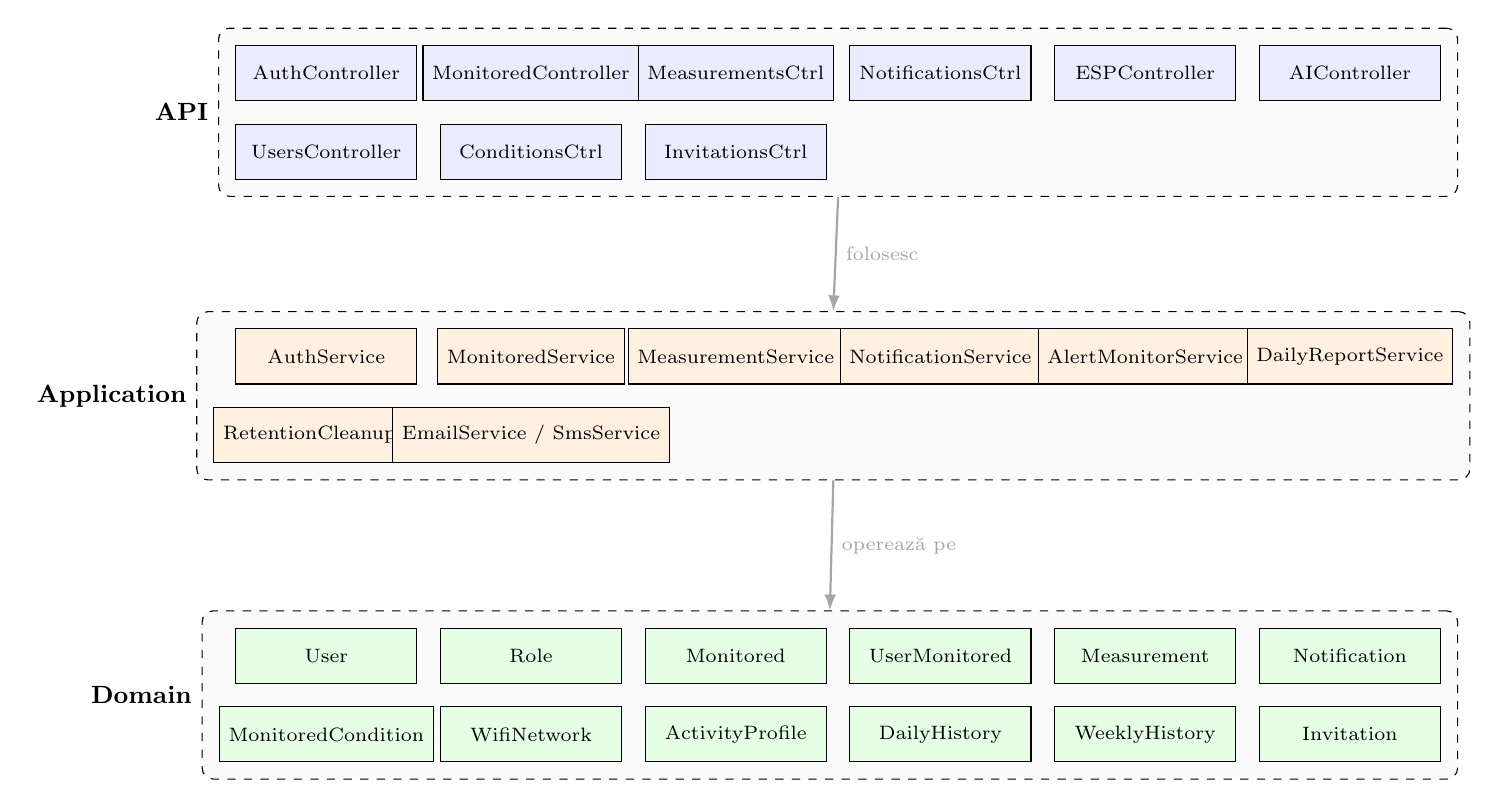
\begin{tikzpicture}[
    every node/.style={font=\scriptsize},
    layer/.style={rectangle, rounded corners, draw, dashed, inner sep=6pt, fill=gray!4},
    cls/.style={rectangle, draw, minimum width=2.3cm, minimum height=0.7cm, align=center, font=\scriptsize, fill=white},
    ctrl/.style={cls, fill=blue!8},
    svc/.style={cls, fill=orange!12},
    ent/.style={cls, fill=green!10},
    layerlabel/.style={font=\small\bfseries, anchor=east},
    arrow/.style={-{Latex[length=2mm]}, thick, gray!70}]

  \node[ctrl] (cAuth)   at (-6.0, 6.6) {AuthController};
  \node[ctrl] (cMon)    at (-3.4, 6.6) {MonitoredController};
  \node[ctrl] (cMeas)   at (-0.8, 6.6) {MeasurementsCtrl};
  \node[ctrl] (cNotif)  at ( 1.8, 6.6) {NotificationsCtrl};
  \node[ctrl] (cESP)    at ( 4.4, 6.6) {ESPController};
  \node[ctrl] (cAI)     at ( 7.0, 6.6) {AIController};
  \node[ctrl] (cUsers)  at (-6.0, 5.6) {UsersController};
  \node[ctrl] (cCond)   at (-3.4, 5.6) {ConditionsCtrl};
  \node[ctrl] (cInv)    at (-0.8, 5.6) {InvitationsCtrl};

  \begin{scope}[on background layer]
    \node[layer, fit=(cAuth)(cAI)(cUsers)(cInv), label={[layerlabel]left:API}] (apiLayer) {};
  \end{scope}

  \node[svc] (sAuth)  at (-6.0, 3.0) {AuthService};
  \node[svc] (sMon)   at (-3.4, 3.0) {MonitoredService};
  \node[svc] (sMeas)  at (-0.8, 3.0) {MeasurementService};
  \node[svc] (sNotif) at ( 1.8, 3.0) {NotificationService};
  \node[svc] (sAlert) at ( 4.4, 3.0) {AlertMonitorService};
  \node[svc] (sDaily) at ( 7.0, 3.0) {DailyReportService};
  \node[svc] (sRet)   at (-6.0, 2.0) {RetentionCleanupSvc};
  \node[svc] (sExt)   at (-3.4, 2.0) {EmailService / SmsService};

  \begin{scope}[on background layer]
    \node[layer, fit=(sAuth)(sDaily)(sRet)(sExt), label={[layerlabel]left:Application}] (appLayer) {};
  \end{scope}

  \node[ent] (eUser)  at (-6.0,-0.8) {User};
  \node[ent] (eRole)  at (-3.4,-0.8) {Role};
  \node[ent] (eMon)   at (-0.8,-0.8) {Monitored};
  \node[ent] (eUM)    at ( 1.8,-0.8) {UserMonitored};
  \node[ent] (eMeas)  at ( 4.4,-0.8) {Measurement};
  \node[ent] (eNotif) at ( 7.0,-0.8) {Notification};
  \node[ent] (eCond)  at (-6.0,-1.8) {MonitoredCondition};
  \node[ent] (eWifi)  at (-3.4,-1.8) {WifiNetwork};
  \node[ent] (eAct)   at (-0.8,-1.8) {ActivityProfile};
  \node[ent] (eDay)   at ( 1.8,-1.8) {DailyHistory};
  \node[ent] (eWeek)  at ( 4.4,-1.8) {WeeklyHistory};
  \node[ent] (eInv)   at ( 7.0,-1.8) {Invitation};

  \begin{scope}[on background layer]
    \node[layer, fit=(eUser)(eNotif)(eCond)(eInv), label={[layerlabel]left:Domain}] (domLayer) {};
  \end{scope}

  \draw[arrow] (apiLayer.south) -- node[right, midway, font=\scriptsize]{folosesc} (appLayer.north);
  \draw[arrow] (appLayer.south) -- node[right, midway, font=\scriptsize]{operează pe} (domLayer.north);
\end{tikzpicture}}
\caption{Diagrama de clase simplificată a aplicației LifeAlertPlus, organizată pe trei straturi: API (controlere), Application (servicii) și Domain (entități). Săgețile reprezintă direcția dependențelor între straturi.}
\label{fig:clase}
\end{figure}

\subsection{Modelul de date}

Modelul de date al sistemului este alcătuit din douăsprezece entități, fiecare corespunzând unei tabele în baza de date. Entitățile principale și rolul lor sunt următoarele:

\begin{itemize}[leftmargin=1.5em]
\item \textbf{User}: utilizatorul aplicației web (aparținător, medic sau administrator). Conține datele de identificare, credențialele, preferințele de afișare și de notificare (email, push, SMS, raport zilnic), precum și un set de praguri implicite pentru parametrii vitali.
\item \textbf{Role}: rolul unui utilizator, care îi determină drepturile în aplicație.
\item \textbf{Monitored}: persoana monitorizată (pacientul vârstnic). Conține datele personale, numărul de serie al dispozitivului asociat, frecvența de actualizare, \textbf{pragurile de alertă personalizate} pentru puls, temperatură și \spo, precum și \textbf{perioada de retenție a datelor} (în zile), după care măsurătorile, notificările și agregările pacientului sunt șterse definitiv.
\item \textbf{UserMonitored}: tabelă de legătură care modelează relația \textit{mulți-la-mulți} dintre utilizatori și persoanele monitorizate; un utilizator poate monitoriza mai multe persoane, iar o persoană poate fi monitorizată de mai mulți utilizatori (aparținător + medic invitat, de exemplu).
\item \textbf{Measurement}: o măsurătoare individuală transmisă de dispozitiv, cu valorile de puls, temperatură, \spo, activitatea detectată, indicatorul de cădere și coordonatele geografice.
\item \textbf{MonitoredCondition}: o afecțiune medicală preexistentă a unei persoane monitorizate (hipertensiune, aritmie, diabet etc.), folosită de modulul AI pentru ajustarea evaluării.
\item \textbf{ActivityProfile}: profilul de activitate al unei persoane, agregat pe ore ale zilei (puls mediu, rata de mișcare, probabilitatea de somn).
\item \textbf{Notification}: o notificare generată de sistem, asociată unei persoane monitorizate și, opțional, unui utilizator destinatar. Pe lângă conținutul mesajului, înregistrează și \textbf{feedback-ul utilizatorului} cu privire la veridicitatea alertei: dacă alerta a fost rezolvată (vitalele au revenit la normal), notificarea primește un marcaj de solicitare a feedback-ului, iar la următoarea vizită în aplicație utilizatorul răspunde printr-un popup dacă alerta a fost reală sau falsă.
\item \textbf{WifiNetwork}: o rețea WiFi configurată pentru dispozitivul fizic al unei persoane monitorizate (SSID + parolă). O persoană poate avea până la trei rețele înregistrate (de exemplu rețeaua de acasă și un hotspot mobil), pe care dispozitivul le încearcă la conectare în ordinea înregistrării.
\item \textbf{DailyHistory} și \textbf{WeeklyHistory}: date agregate zilnic, respectiv săptămânal (valori minime/maxime, medii, numărul de căderi și de alerte), folosite pentru rapoarte și statistici.
\item \textbf{Invitation}: o invitație trimisă unui medic pentru a-i acorda acces la datele unui pacient, identificată printr-un token unic cu termen de expirare.
\end{itemize}

\subsubsection{Relațiile dintre entități}

Relația centrală a modelului este cea \textit{mulți-la-mulți} dintre \texttt{User} și \texttt{Monitored}, realizată prin tabela de legătură \texttt{UserMonitored}, a cărei cheie primară este compusă din cele două chei străine. Fiecare persoană monitorizată este, totodată, în relație \textit{unu-la-mulți} cu măsurătorile, notificările, afecțiunile, profilele de activitate și înregistrările de istoric care îi aparțin. Ștergerea unei persoane monitorizate determină ștergerea în cascadă a datelor sale dependente, în timp ce relațiile cu utilizatorii sunt protejate la ștergere, pentru a păstra integritatea referențială.

Pentru a optimiza performanța interogărilor frecvente, au fost definite indexuri pe cheile străine cele mai utilizate, în special pe identificatorul persoanei monitorizate din tabelele de măsurători și notificări. Token-ul fiecărei invitații este indexat unic, iar combinația dintre o persoană monitorizată și o afecțiune este, de asemenea, unică, pentru a împiedica înregistrările duplicate.

\subsubsection{Ștergerea datelor}

Sistemul folosește două politici complementare de ștergere, în funcție de tipul datelor. Pentru entitățile cu rol identitar, anume \texttt{User} și \texttt{Monitored}, se aplică \textbf{ștergere logică} (soft delete): înregistrările primesc o dată în câmpul \texttt{DeletedAt} și sunt excluse din interogările obișnuite, păstrând astfel integritatea istoricului medical și permițând recuperarea în caz de eroare. Pentru entitățile de tip volumetric, anume \texttt{Measurement}, \texttt{Notification}, \texttt{DailyHistory} și \texttt{WeeklyHistory}, se aplică \textbf{ștergere fizică} (hard delete) prin \textit{job-ul} zilnic de retenție descris în subcapitolul 4.4: înregistrările mai vechi decât perioada configurată (\texttt{DataRetentionDays} de pe persoana monitorizată) sunt eliminate definitiv, atât pentru a respecta principiul minimizării datelor cerut de regulamentul GDPR, cât și pentru a limita creșterea bazei de date sub fluxul continuu de măsurători de la dispozitiv.

\subsubsection{Datele agregate și istoricul}

Pe lângă entitățile care reflectă starea curentă, modelul include entități de \textbf{date agregate}, calculate periodic din măsurătorile brute. \texttt{DailyHistory} reține, pentru fiecare zi, valorile minime și maxime ale pulsului și temperaturii, numărul de căderi și numărul de alerte; \texttt{WeeklyHistory} reține medii și totaluri la nivel de săptămână. Aceste entități nu adaugă informație nouă, ci o sintetizează: ele permit afișarea rapidă a statisticilor și generarea rapoartelor fără a parcurge de fiecare dată întregul istoric de măsurători, care crește considerabil în timp. O a treia formă de agregare este \texttt{ActivityProfile}, care reține distribuția activității pacientului pe orele zilei și stă la baza profilului de activitate zilnică.

Diagrama entitate-relație a modelului de date este prezentată în figura~\ref{fig:model-date}.

\begin{figure}[H]
\centering
\resizebox{\textwidth}{!}{%
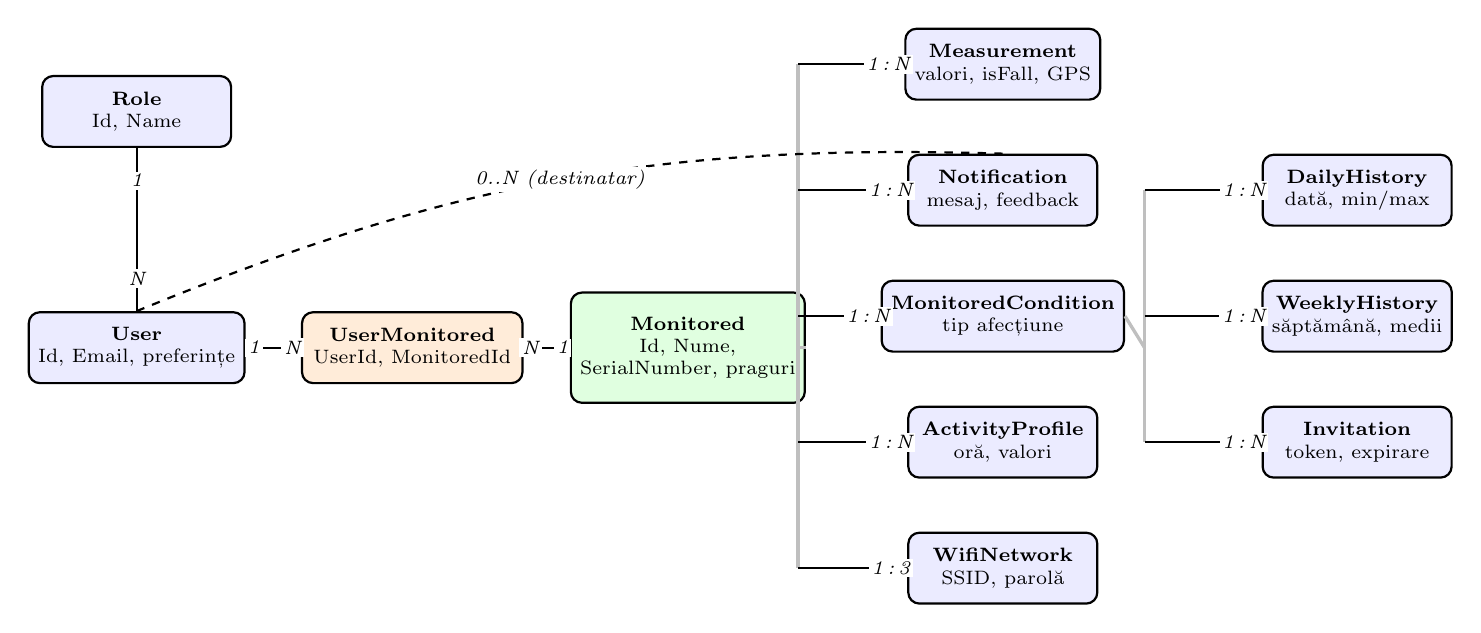
\begin{tikzpicture}[
    every node/.style={font=\scriptsize},
    ent/.style={rectangle, rounded corners, draw, thick, minimum width=2.4cm, minimum height=0.9cm, align=center, fill=blue!8},
    link/.style={rectangle, rounded corners, draw, thick, minimum width=2.8cm, minimum height=0.9cm, align=center, fill=orange!15},
    central/.style={rectangle, rounded corners, draw, thick, minimum width=2.6cm, minimum height=1.4cm, align=center, fill=green!12},
    rel/.style={draw, thick},
    bus/.style={draw, very thick, gray!50},
    card/.style={font=\scriptsize\itshape, fill=white, inner sep=1pt}]

  \node[ent] (role) at (-7.0, 3.0) {\textbf{Role}\\\scriptsize Id, Name};
  \node[ent] (user) at (-7.0, 0.0) {\textbf{User}\\\scriptsize Id, Email, preferințe};

  \node[link] (um) at (-3.5, 0.0) {\textbf{UserMonitored}\\\scriptsize UserId, MonitoredId};

  \node[central] (mon) at (0.0, 0.0) {\textbf{Monitored}\\\scriptsize Id, Nume,\\\scriptsize SerialNumber, praguri};

  \def\yMeas{3.6}
  \def\yNotif{2.0}
  \def\yCond{0.4}
  \def\yAct{-1.2}
  \def\yWifi{-2.8}
  \def\yDay{2.0}
  \def\yWeek{0.4}
  \def\yInv{-1.2}

  \node[ent] (meas)  at ( 4.0, \yMeas)  {\textbf{Measurement}\\\scriptsize valori, isFall, GPS};
  \node[ent] (notif) at ( 4.0, \yNotif) {\textbf{Notification}\\\scriptsize mesaj, feedback};
  \node[ent] (cond)  at ( 4.0, \yCond)  {\textbf{MonitoredCondition}\\\scriptsize tip afecțiune};
  \node[ent] (act)   at ( 4.0, \yAct)   {\textbf{ActivityProfile}\\\scriptsize oră, valori};
  \node[ent] (wifi)  at ( 4.0, \yWifi)  {\textbf{WifiNetwork}\\\scriptsize SSID, parolă};

  \node[ent] (day)   at ( 8.5, \yDay)  {\textbf{DailyHistory}\\\scriptsize dată, min/max};
  \node[ent] (week)  at ( 8.5, \yWeek) {\textbf{WeeklyHistory}\\\scriptsize săptămână, medii};
  \node[ent] (inv)   at ( 8.5, \yInv)  {\textbf{Invitation}\\\scriptsize token, expirare};

  \draw[rel] (role.south) -- node[card, pos=0.2]{1} node[card, pos=0.8]{N} (user.north);
  \draw[rel] (user.east)  -- node[card, pos=0.15]{1} node[card, pos=0.85]{N} (um.west);
  \draw[rel] (um.east)    -- node[card, pos=0.15]{N} node[card, pos=0.85]{1} (mon.west);

  \coordinate (bus) at (1.4,0);
  \draw[bus] (mon.east) -- (bus);
  \draw[bus] (1.4,\yWifi) -- (1.4,\yMeas);

  \draw[rel] (1.4,\yMeas)  -- node[card, pos=0.85]{1\,:\,N} (meas.west);
  \draw[rel] (1.4,\yNotif) -- node[card, pos=0.85]{1\,:\,N} (notif.west);
  \draw[rel] (1.4,\yCond)  -- node[card, pos=0.85]{1\,:\,N} (cond.west);
  \draw[rel] (1.4,\yAct)   -- node[card, pos=0.85]{1\,:\,N} (act.west);
  \draw[rel] (1.4,\yWifi)  -- node[card, pos=0.85]{1\,:\,3} (wifi.west);

  \coordinate (bus2) at (5.8,0);
  \draw[bus] (5.8,\yInv) -- (5.8,\yDay);
  \draw[bus] (cond.east) -- (bus2);
  \draw[rel] (5.8,\yDay)  -- node[card, pos=0.85]{1\,:\,N} (day.west);
  \draw[rel] (5.8,\yWeek) -- node[card, pos=0.85]{1\,:\,N} (week.west);
  \draw[rel] (5.8,\yInv)  -- node[card, pos=0.85]{1\,:\,N} (inv.west);

  \draw[rel, dashed] (user.north) to[bend left=12] node[card, pos=0.5]{0..N (destinatar)} (notif.north);
\end{tikzpicture}}
\caption{Diagrama entitate-relație a bazei de date LifeAlertPlus. Relația centrală \textit{mulți-la-mulți} dintre \texttt{User} și \texttt{Monitored} se realizează prin tabela de legătură \texttt{UserMonitored}. Toate entitățile dependente sunt legate \textit{unu-la-mulți} de \texttt{Monitored}, iar relația punctată indică o legătură opțională (un destinatar pentru o notificare).}
\label{fig:model-date}
\end{figure}

\subsection{Fluxuri de funcționare}

\subsubsection{Achiziția și transmiterea unei măsurători}

Fluxul principal al sistemului începe pe dispozitivul portabil. La intervalul de timp configurat, microcontrollerul citește valorile tuturor senzorilor, filtrează citirile evident eronate și calculează mărimile derivate (pulsul, magnitudinea acceleraţiei, etc.). Pachetul de date rezultat, care include și un \textbf{indicator boolean} setat în cazul în care detectorul de căderi a confirmat un eveniment de cădere, este transmis backend-ului printr-o cerere HTTP către endpoint-ul de ingestie, autentificată printr-o cheie de dispozitiv transmisă în antetul cererii. Dacă transmiterea eșuează din cauza lipsei conexiunii, măsurătoarea este adăugată în coada locală a dispozitivului și retransmisă ulterior. La recepție, backend-ul validează cheia de dispozitiv, asociază măsurătoarea persoanei monitorizate pe baza numărului de serie, o persistă în baza de date și o transmite mai departe serviciului de monitorizare a alertelor împreună cu indicatorul de cădere; o cădere raportată de dispozitiv ridică automat severitatea evaluării la nivel critic, indiferent de valorile parametrilor vitali.

\subsubsection{Evaluarea stării prin modulul AI}

Fiecare măsurătoare primită este trimisă microserviciului de inteligență artificială, împreună cu pragurile personalizate ale pacientului și lista afecțiunilor sale. Microserviciul returnează starea prezisă, health score-ul și explicația. Pentru a evita ca o indisponibilitate a serviciului AI să blocheze fluxul, cererea are un timp de așteptare scurt, iar în lipsa unui răspuns sistemul recurge la evaluarea pe bază de reguli.

\subsubsection{Calculul health score-ului}

Health score-ul este un indice numeric între 0 și 100, în care valoarea 0 corespunde unei stări complet stabile, iar valori ridicate corespund unui risc crescut. Spre deosebire de o alertă bazată pe depășirea unui singur prag, health score-ul este o \textbf{sumă ponderată de contribuții}, fiecare parametru vital adăugând la scor o cantitate proporțională cu severitatea abaterii sale. Pragurile utilizate sunt cele personalizate ale pacientului, cu valori clinice implicite atunci când acestea nu au fost configurate.

Contribuțiile sunt agregate astfel:

\begin{itemize}[leftmargin=1.5em]
\item \textbf{Saturația oxigenului} are ponderea cea mai mare: o valoare sub pragul critic adaugă o contribuție majoră, iar o valoare situată între pragul critic și cel minim adaugă o contribuție proporțională cu distanța față de prag.
\item \textbf{Frecvența cardiacă} adaugă o contribuție mare la depășirea pragului maxim sau la coborârea sub cel minim și o contribuție moderată în zonele de avertizare aflate înaintea acestor praguri.
\item \textbf{Temperatura corporală} contribuie similar, atât pentru valori febrile, cât și pentru hipotermie.
\item \textbf{Imobilitatea}, manifestată prin accelerație foarte redusă, care poate indica o cădere urmată de imobilizare, adaugă o contribuție suplimentară.
\item \textbf{Afecțiunile preexistente} aplică modificatori specifici: de exemplu, în cazul unei aritmii, un puls anormal adaugă o penalizare suplimentară, întrucât are o semnificație clinică mai gravă pentru acel pacient.
\end{itemize}

Ponderile concrete utilizate în agregare sunt sintetizate în tabelul~\ref{tab:healthscore}. Pragurile la care se raportează condițiile sunt cele personalizate ale pacientului; în lipsa configurării, se folosesc valori clinice implicite (frecvență cardiacă 50--130 bpm, temperatură 35--39\,\textdegree C, saturație minimă 95\%).

\begin{table}[H]
\centering
\small
\renewcommand{\arraystretch}{1.3}
\begin{tabular}{|>{\raggedright\arraybackslash}p{3.0cm}|>{\raggedright\arraybackslash}p{7.2cm}|c|}
\hline
\textbf{Parametru} & \textbf{Condiție} & \textbf{Contribuție}\\
\hline
\multicolumn{3}{|l|}{\textit{Parametri vitali}}\\
\hline
\spo & Sub pragul critic de saturație & $+60$\\
\hline
\spo & Între pragul critic și pragul minim & $+30$ (gradual)\\
\hline
Frecvență cardiacă & Peste pragul maxim & $+25$\\
\hline
Frecvență cardiacă & Zona de avertizare înaltă (peste 85\% din maxim) & $+12$\\
\hline
Frecvență cardiacă & Sub pragul minim & $+20$\\
\hline
Frecvență cardiacă & Zona de avertizare joasă (sub 120\% din minim) & $+10$\\
\hline
Temperatură corporală & Peste pragul maxim & $+20$\\
\hline
Temperatură corporală & Zona de avertizare înaltă (cu 1\,\textdegree C sub maxim) & $+10$\\
\hline
Temperatură corporală & Sub pragul minim & $+20$\\
\hline
Temperatură corporală & Zona de avertizare joasă (cu 1\,\textdegree C peste minim) & $+10$\\
\hline
Imobilitate & Accelerație sub 0,2\,g (posibilă cădere/imobilizare) & $+8$\\
\hline
\multicolumn{3}{|l|}{\textit{Modificatori în funcție de afecțiunile preexistente}}\\
\hline
Hipertensiune & Puls peste 100 bpm & $+8$\\
\hline
Aritmie & Puls peste 110 bpm sau sub 52 bpm & $+10$\\
\hline
Risc de infarct & Puls peste 110 bpm și temperatură peste 37,8\,\textdegree C & $+12$\\
\hline
Diabet & Temperatură peste 38\,\textdegree C & $+8$\\
\hline
Parkinson / epilepsie & Accelerație sub 0,5\,g & $+5$\\
\hline
\end{tabular}
\caption{Ponderile contribuțiilor în calculul health score-ului.}
\label{tab:healthscore}
\end{table}

Scorul rezultat este limitat la intervalul $[0, 100]$. Avantajul acestui mecanism este că surprinde \textbf{corelația dintre mai mulți parametri}: mai multe abateri ușoare, fiecare insuficientă pentru a declanșa singură o alertă, se pot cumula într-un scor ridicat, semnalând o degradare globală a stării pacientului care altfel ar trece neobservată.

\subsubsection{Predicția de tendințe}

Pe lângă evaluarea stării instantanee, sistemul oferă o \textbf{predicție de tendințe pe termen scurt}, menită să anticipeze atingerea unui prag clinic înainte ca acesta să fie efectiv depășit. Serviciul de monitorizare păstrează, pentru fiecare pacient, un buffer cu măsurătorile din ultimele două minute și calculează, pentru fiecare parametru vital (puls, temperatură, \spo), media și \textbf{panta} (rata de variație) pe acest interval. Atunci când panta indică o evoluție constantă către o valoare critică, sistemul estimează timpul rămas până la atingerea pragului prin extrapolare liniară și produce o etichetă explicativă.

De exemplu, o temperatură în creștere constantă generează predicția \textit{Posibilă febră} sau \textit{Febră în evoluție}, împreună cu numărul aproximativ de secunde până la pragul de 38,5\,\textdegree C; analog, se anticipează tahicardia, bradicardia sau hipoxia. Aceste predicții sunt afișate în interfața de vizualizare a pacientului (figura~\ref{fig:predictii-tendinte}) ca avertismente gradate (atenționare sau pericol) și au rol pur informativ pentru aparținător, fără a declanșa singure notificări, întrucât se bazează pe extrapolare și nu pe o depășire efectivă a pragului. Spre deosebire de health score, care reflectă starea curentă, predicția de tendințe priveşte în viitorul apropiat (de ordinul minutelor).

\begin{figure}[H]
\centering
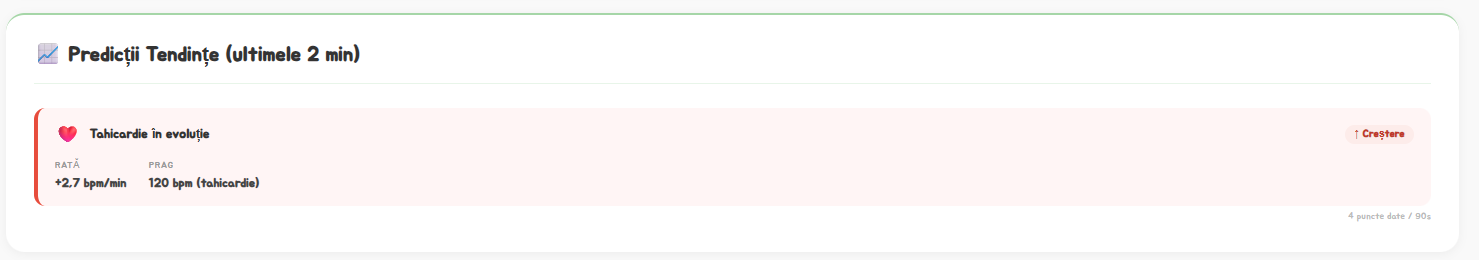
\includegraphics[width=\textwidth]{figuri/predictii-tendinte.png}
\caption{Predicțiile de tendințe afișate în pagina pacientului: etichetă, valoare curentă, rată de variație și timp estimat până la prag.}
\label{fig:predictii-tendinte}
\end{figure}

\subsubsection{Declanșarea și escaladarea unei alerte}

Detectarea unei situații de risc nu declanșează imediat o notificare. Serviciul de monitorizare a alertelor menține, pentru fiecare persoană monitorizată, un buffer cu măsurătorile recente și aplică un \textbf{prag de persistență}: o stare anormală trebuie să se mențină o durată minimă înainte de a genera o alertă, eliminând astfel valorile tranzitorii cauzate de un contact imperfect al senzorului. Severitatea de bază a alertei este apoi ajustată de motorul de reguli pe baza afecțiunilor pacientului, care poate ridica nivelul de severitate și poate adăuga recomandări specifice.

Odată confirmată, alerta este livrată simultan prin toate canalele activate în preferințele aparținătorului, anume notificare push, email și/sau SMS. Pragul de persistență este de aproximativ două minute în cazul stărilor critice; după ce este atins, toate canalele alese de utilizator primesc notificarea în același moment, fără ca SMS-ul să fie întârziat suplimentar față de celelalte. Atâta vreme cât starea critică persistă, sistemul retrimite notificarea la fiecare două minute; pentru alertele non-critice, un mecanism de \textbf{cooldown} împiedică retransmiterea aceleiași alerte pentru aceeași persoană într-un interval scurt, evitând inundarea destinatarului cu mesaje. În cazul alertelor critice, sistemul include în notificare și informații despre cel mai apropiat spital față de poziția pacientului. Întregul flux, de la achiziția măsurătorii până la livrarea alertei, este ilustrat în figura~\ref{fig:flux-alerta}.

\begin{figure}[H]
\centering
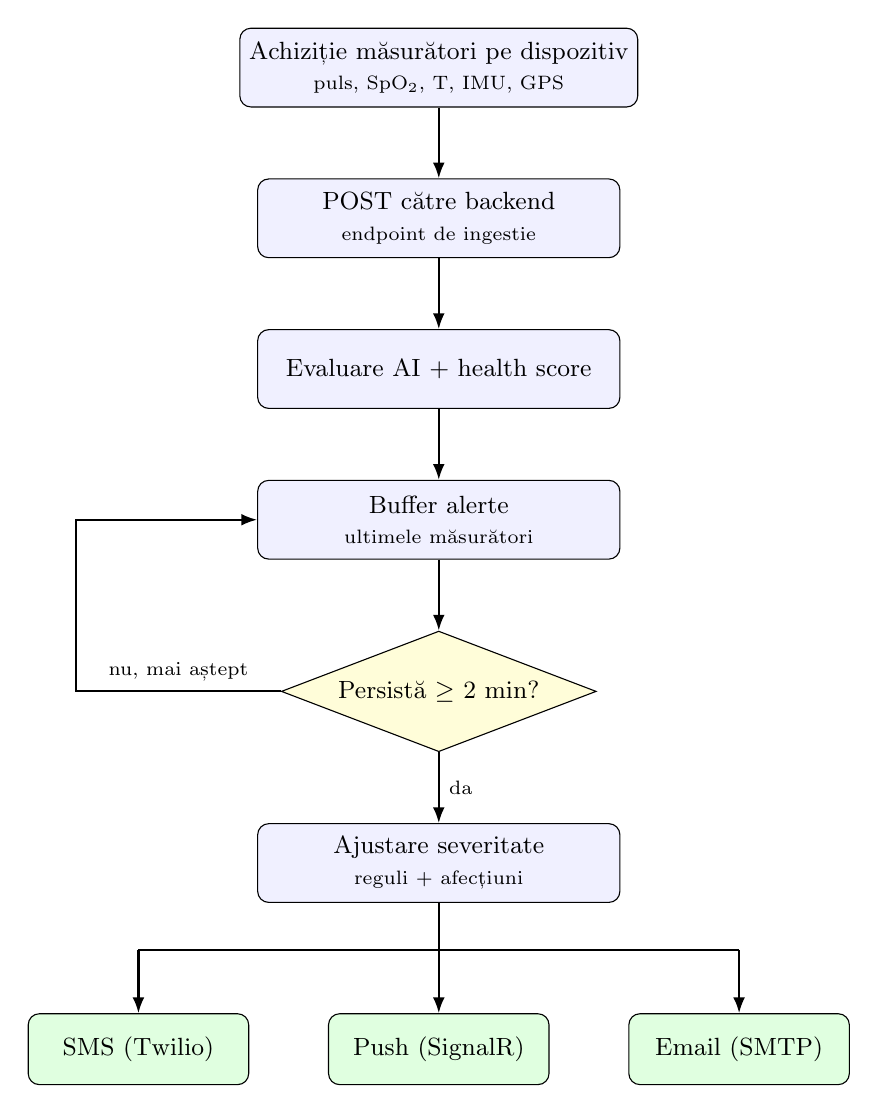
\begin{tikzpicture}[node distance=0.9cm and 1.0cm,
    every node/.style={font=\small},
    box/.style={rectangle, rounded corners, draw, minimum width=4.6cm, minimum height=1.0cm, align=center, fill=blue!6},
    decide/.style={diamond, aspect=2.4, draw, align=center, fill=yellow!15, inner sep=2pt, minimum width=4.0cm},
    outp/.style={rectangle, rounded corners, draw, minimum width=2.8cm, minimum height=0.9cm, align=center, fill=green!12},
    arrow/.style={-{Latex[length=2mm]}, thick},
    label/.style={font=\scriptsize}]

  \node[box] (sens) {Achiziție măsurători pe dispozitiv\\\scriptsize puls, \spo, T, IMU, GPS};
  \node[box, below=of sens] (post) {POST către backend\\\scriptsize endpoint de ingestie};
  \node[box, below=of post] (ai) {Evaluare AI + health score};
  \node[box, below=of ai] (buf) {Buffer alerte\\\scriptsize ultimele măsurători};
  \node[decide, below=of buf] (pers) {Persistă $\geq$ 2 min?};
  \node[box, below=of pers] (sev) {Ajustare severitate\\\scriptsize reguli + afecțiuni};
  \node[outp, below=1.4cm of sev] (push) {Push (SignalR)};
  \node[outp, left=of push] (sms) {SMS (Twilio)};
  \node[outp, right=of push] (mail) {Email (SMTP)};

  \draw[arrow] (sens) -- (post);
  \draw[arrow] (post) -- (ai);
  \draw[arrow] (ai) -- (buf);
  \draw[arrow] (buf) -- (pers);
  \draw[arrow] (pers) -- node[right, label]{da} (sev);

  \draw[arrow] (pers.west) -- ++(-2.6,0) node[midway, above, label]{nu, mai aștept} |- (buf.west);

  \coordinate (junc) at ($(sev.south) + (0,-0.6)$);
  \draw[thick] (sev.south) -- (junc);
  \draw[thick] (sms.north |- junc) -- (mail.north |- junc);
  \draw[arrow] (sms.north |- junc) -- (sms.north);
  \draw[arrow] (push.north |- junc) -- (push.north);
  \draw[arrow] (mail.north |- junc) -- (mail.north);
\end{tikzpicture}
\caption{Fluxul de declanșare și escaladare a unei alerte.}
\label{fig:flux-alerta}
\end{figure}

\subsubsection{Butonul de panică}

Independent de fluxul automat, pacientul poate declanșa el însuși o alertă apăsând butonul de panică al dispozitivului. Această acțiune trimite o cerere dedicată către backend, care generează imediat o alertă către aparținător, fără a aștepta pragul de persistență și indiferent de valorile senzorilor, întrucât reprezintă o solicitare explicită de ajutor. Mesajul livrat aparținătorului specifică explicit faptul că \textit{vârstnicul nu se simte în siguranță} și a apăsat butonul de panică, iar livrarea se face prin \textbf{toate canalele activate în preferințele aparținătorului} (notificare push, email și SMS), pentru a maximiza probabilitatea de a fi observat imediat. Dacă dispozitivul are un fix GPS valid în momentul apăsării, notificarea include și ultima poziție cunoscută a pacientului, împreună cu informații despre cel mai apropiat spital de urgență. În caz de pierdere temporară a conexiunii, alerta de panică este salvată într-o coadă locală separată de cea a măsurătorilor obișnuite și are prioritate la retransmitere când conexiunea revine.

\subsubsection{Detecția căderilor pe dispozitiv}

Detecția căderilor este realizată \textbf{integral pe dispozitiv}, ca task separat care eșantionează accelerometrul MPU6050 la o frecvență de aproximativ 50\,Hz. Algoritmul, bazat pe trecerea acceleraţiei prin trei faze succesive, este implementat ca o mașină de stări cu trei stări active: \textit{IDLE}, \textit{IN\_FREEFALL} și \textit{MONITORING\_STILLNESS}. Pentru fiecare eșantion se calculează magnitudinea vectorului de acceleraţie, $|\vec{a}| = \sqrt{a_x^2 + a_y^2 + a_z^2}$, și se aplică tranziţiile prezentate în figura~\ref{fig:fall-state}.

\begin{figure}[H]
\centering
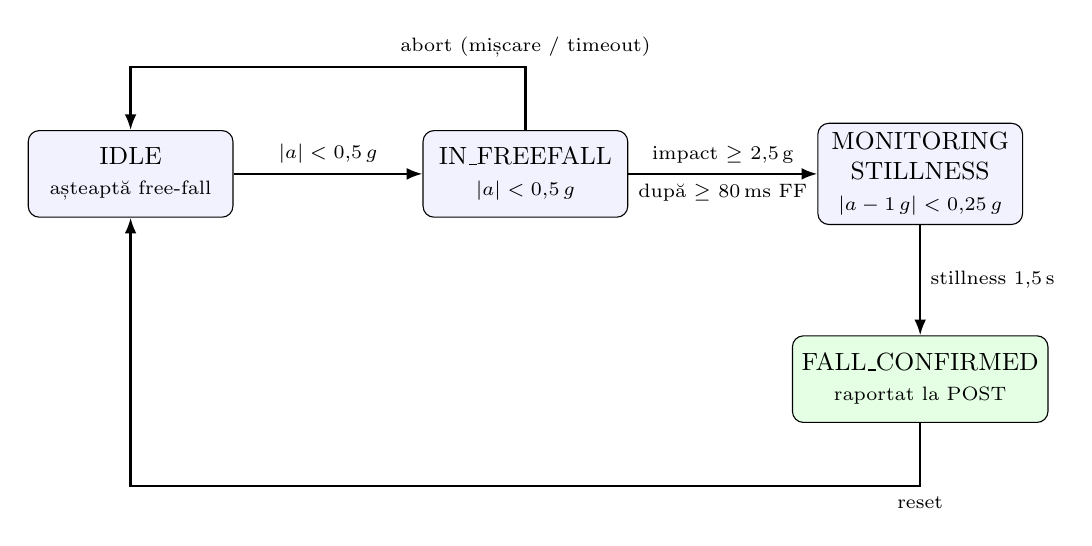
\begin{tikzpicture}[node distance=1.4cm and 2.4cm,
    every node/.style={font=\small},
    state/.style={rectangle, rounded corners, draw, minimum width=2.6cm, minimum height=1.1cm, align=center, fill=blue!5},
    edge/.style={-{Latex[length=2mm]}, thick}]

  \node[state] (idle) {IDLE\\\scriptsize așteaptă free-fall};
  \node[state, right=of idle] (ff) {IN\_FREEFALL\\\scriptsize $|a| < 0{,}5\,g$};
  \node[state, right=of ff] (st) {MONITORING\\STILLNESS\\\scriptsize $|a - 1\,g| < 0{,}25\,g$};
  \node[state, below=of st, fill=green!10] (conf) {FALL\_CONFIRMED\\\scriptsize raportat la POST};

  \draw[edge] (idle) -- node[above, font=\scriptsize]{$|a| < 0{,}5\,g$} (ff);
  \draw[edge] (ff) -- node[above, font=\scriptsize]{impact $\geq$ 2{,}5\,g} node[below, font=\scriptsize]{după $\geq$ 80\,ms FF} (st);
  \draw[edge] (st) -- node[right, font=\scriptsize]{stillness 1{,}5\,s} (conf);

  \draw[edge] (ff.north) -- ++(0,0.8) node[above, font=\scriptsize]{abort (mișcare / timeout)} -| (idle.north);

  \draw[edge] (conf.south) -- ++(0,-0.8) node[below, font=\scriptsize]{reset} -| (idle.south);
\end{tikzpicture}
\caption{Mașina de stări a detectorului de căderi rulat pe dispozitiv.}
\label{fig:fall-state}
\end{figure}

Pragurile au fost alese empiric pe baza literaturii de specialitate pentru detectori de tip prag: free-fall sub 0,5\,g susținut minim 80\,ms, impact peste 2,5\,g într-o fereastră de cel mult 800\,ms după free-fall, urmat de o perioadă de stillness de 1,5\,s în care magnitudinea acceleraţiei rămâne în jurul valorii de 1\,g (gravitaţia), cu variaţii sub 0,25\,g. La confirmare, task-ul setează un flag pe care bucla principală îl include în următoarea cerere către endpoint-ul de ingestie. Fluxul restant se identifică cu cel al unei măsurători obișnuite, însă serverul ridică automat severitatea la nivel critic atunci când indicatorul de cădere este activ, declanșând livrarea pe toate canalele activate.

\subsubsection{Profilul de activitate și detecția anomaliilor comportamentale}

Pe lângă măsurătorile instantanee, sistemul construiește pentru fiecare pacient un \textbf{profil de activitate zilnică} agregat pe orele zilei dintr-o fereastră glisantă de 7 zile. Sursa de date este eticheta de activitate (\texttt{moving} / \texttt{stationary}) calculată în firmware pentru fiecare măsurătoare (procedeu descris în subcapitolul de implementare a firmware-ului). Pentru fiecare oră a zilei, serviciul de profilare păstrează trei valori derivate: pulsul mediu, \textbf{rata de mişcare} (proporţia măsurătorilor etichetate \texttt{moving}) şi \textbf{probabilitatea de somn} (proporţia măsurătorilor etichetate \texttt{stationary} la care pulsul este sub 75\,bpm). Profilul este recalculat în fundal o singură dată per pacient, atunci când e folosit prima oară, şi păstrat într-o memorie locală cu expirare la 4 ore pentru a evita interogări repetate pe baza de date.

Pe baza acestui profil, la fiecare măsurătoare nouă serviciul de monitorizare verifică dacă starea curentă se abate semnificativ de la tiparul obişnuit al pacientului la ora respectivă, declanşând una dintre două \textbf{anomalii comportamentale}:

\begin{itemize}[leftmargin=1.5em]
\item \textbf{Inactivitate prelungită}: în ultimele 15 minute toate măsurătorile au fost etichetate \texttt{stationary}, deşi la ora curentă pacientul se mişcă în mod obişnuit cel puţin 65\% din timp (după profilul de 7 zile). Acest scenariu poate semnala o situaţie de risc (cădere nedetectată, leşin, imobilizare).
\item \textbf{Activitate nocturnă}: măsurătoarea curentă este etichetată \texttt{moving} într-o oră în care pacientul doarme de obicei cel puţin 70\% din timp. Acest scenariu poate semnala agitaţie nocturnă, ridicare neaşteptată sau o stare alterată.
\end{itemize}

Atât profilul cât şi detecţia anomaliilor sunt activate numai dacă există suficiente date istorice pentru ora respectivă (minim 20 de măsurători); pentru pacienţi nou înregistraţi mecanismul rămâne inactiv până se acumulează suficiente date pentru un profil semnificativ statistic. Notificările comportamentale sunt limitate prin acelaşi mecanism de \textit{cooldown} (minim 30 de minute între două notificări de acelaşi tip pentru acelaşi pacient) ca să evite inundarea aparţinătorului.

\subsubsection{Configurarea rețelelor WiFi de la distanță}

Pentru a permite folosirea dispozitivului în mai multe medii (de exemplu, acasă și pe un hotspot mobil), aparținătorul poate înregistra din aplicația web până la trei rețele WiFi asociate dispozitivului unui pacient. Lista este persistată în baza de date; dispozitivul interoghează periodic backend-ul pentru ultima configurație disponibilă, în paralel cu \textit{heartbeat-ul} obișnuit. Atunci când configurația citită diferă de cea salvată local pe dispozitiv, lista este rescrisă în memoria nevolatilă (evitând astfel uzura memoriei flash), iar rețelele noi devin active la următoarea repornire a dispozitivului, fără a întrerupe sesiunea curentă. Fluxul complet este ilustrat în figura~\ref{fig:wifi-flow}.

\begin{figure}[H]
\centering
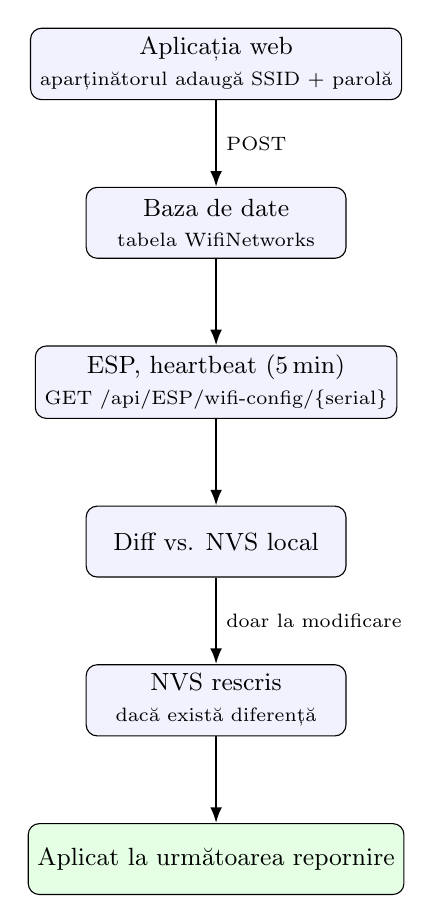
\begin{tikzpicture}[node distance=1.1cm and 2.0cm,
    every node/.style={font=\small},
    box/.style={rectangle, rounded corners, draw, minimum width=3.3cm, minimum height=0.9cm, align=center, fill=blue!5},
    arrow/.style={-{Latex[length=2mm]}, thick}]

  \node[box] (ui) {Aplicația web\\\scriptsize{aparținătorul adaugă SSID + parolă}};
  \node[box, below=of ui] (db) {Baza de date\\\scriptsize{tabela WifiNetworks}};
  \node[box, below=of db] (hb) {ESP, heartbeat (5\,min)\\\scriptsize{GET /api/ESP/wifi-config/\{serial\}}};
  \node[box, below=of hb] (diff) {Diff vs. NVS local};
  \node[box, below=of diff] (nvs) {NVS rescris\\\scriptsize{dacă există diferență}};
  \node[box, below=of nvs, fill=green!10] (boot) {Aplicat la următoarea repornire};

  \draw[arrow] (ui) -- node[right]{\scriptsize POST} (db);
  \draw[arrow] (db) -- (hb);
  \draw[arrow] (hb) -- (diff);
  \draw[arrow] (diff) -- node[right]{\scriptsize doar la modificare} (nvs);
  \draw[arrow] (nvs) -- (boot);
\end{tikzpicture}
\caption{Fluxul de sincronizare a configurației WiFi între aplicația web și dispozitivul fizic.}
\label{fig:wifi-flow}
\end{figure}

\subsubsection{Feedback pentru alarme false}

Pentru a permite ajustarea pragurilor și pentru a oferi date concrete despre rata de alerte false, sistemul implementează o \textbf{buclă de feedback} cu utilizatorul aparținător. Atunci când o stare de alertă (puls anormal, temperatură ridicată, \spo scăzut etc.) se rezolvă, adică valorile pacientului revin la normal după ce o notificare a fost deja trimisă, ultima notificare a episodului este marcată automat ca \textit{așteptând feedback}. La următoarea vizită a aparținătorului în aplicație, un popup neintruziv afișează informațiile alertei (pacient, momentul evenimentului) și întreabă explicit dacă alerta a fost reală sau o alarmă falsă. Răspunsul este înregistrat pe notificare și permite raportarea ulterioară a ratei reale de alerte false, calculată din datele etichetate de utilizator. Utilizatorul poate amâna răspunsul, caz în care popup-ul reapare la următoarea sesiune.

\subsubsection{Politica de retenție a datelor}

Aplicația implementează o politică de retenție configurabilă \textbf{per pacient}. Pentru fiecare persoană monitorizată, aparținătorul poate alege durata maximă de păstrare a datelor (30, 90, 180 sau 365 de zile) din modalul de editare al pacientului. Un \textit{job} de fundal rulează automat o dată pe zi, la miezul nopții (ora locală configurată în setările serverului), și șterge definitiv din baza de date toate măsurătorile, notificările și agregările zilnice / săptămânale mai vechi decât perioada configurată. Spre deosebire de ștergerea logică folosită pentru entitățile cu rol identitar, această curățare este o ștergere fizică ireversibilă, motivată de respectarea principiului de minimizare a datelor și de limitarea creșterii bazei de date sub fluxul continuu de măsurători de la dispozitiv.

\subsubsection{Sincronizarea datelor stocate local}

Atunci când dispozitivul funcționează fără conexiune la internet, măsurătorile se acumulează în coada locală. La revenirea conexiunii, dispozitivul transmite măsurătorile aflate în așteptare, în ordinea înregistrării lor. Astfel, istoricul medical rămâne complet chiar și în condiții de conectivitate intermitentă, în concordanță cu cerința de fiabilitate a sistemelor IoMT prezentată în subcapitolul 2.1.

\subsubsection{Înrolarea utilizatorilor și asocierea dispozitivului}

Înainte de a putea monitoriza o persoană, un aparținător își creează un cont și îl confirmă prin email. Ulterior, el adaugă o persoană monitorizată, completând datele acesteia și asociind numărul de serie al dispozitivului fizic. Această asociere este cheia pe baza căreia backend-ul leagă, ulterior, fiecare măsurătoare primită de la dispozitiv de persoana corectă. Tot la acest moment sunt configurate pragurile de alertă personalizate și afecțiunile preexistente, care vor fi folosite la evaluarea stării de sănătate.

\subsubsection{Invitarea medicului și exportul datelor}

Un aparținător poate acorda unui medic acces la datele unei persoane monitorizate. Sistemul generează în acest scop o invitație identificată printr-un token unic, cu termen de expirare, transmisă medicului prin email; la acceptarea ei, medicul primește drept de vizualizare asupra datelor pacientului respectiv. În plus, istoricul de măsurători poate fi exportat în mod structurat și transmis medicului curant, pentru un interval de timp selectabil, facilitând consultarea datelor în afara aplicației.


\newpage
\phantomsection
\addcontentsline{toc}{section}{Bibliografie}
\begin{thebibliography}{99}

\bibitem{who2023} World Health Organization, \textit{Noncommunicable diseases. Fact sheet}, 2023. \url{https://www.who.int/news-room/fact-sheets/detail/noncommunicable-diseases}.

\bibitem{fbi2023} Fortune Business Insights, \textit{Internet of Medical Things (IoMT) Market Size, Share \& Industry Analysis}, 2023. \url{https://www.fortunebusinessinsights.com/internet-of-medical-things-iomt-market-101844}.

\bibitem{ashton1999} K. Ashton, \textit{That ``Internet of Things'' Thing}, RFID Journal, 1999. \url{https://www.rfidjournal.com/that-internet-of-things-thing}.

\bibitem{lundberg2017} S. M. Lundberg, S.-I. Lee, \textit{A Unified Approach to Interpreting Model Predictions}, în Advances in Neural Information Processing Systems (NeurIPS), 2017. \url{https://proceedings.neurips.cc/paper_files/paper/2017/hash/8a20a8621978632d76c43dfd28b67767-Abstract.html}.

\bibitem{scikit} F. Pedregosa et al., \textit{Scikit-learn: Machine Learning in Python}, Journal of Machine Learning Research, vol. 12, pp. 2825--2830, 2011. \url{https://www.jmlr.org/papers/v12/pedregosa11a.html}.

\bibitem{bidmc} PhysioNet, \textit{BIDMC PPG and Respiration Dataset}, v1.0.0. \url{https://physionet.org/content/bidmc/1.0.0/}.

\bibitem{espressif} Espressif Systems, \textit{ESP32-C3 Series Datasheet}. \url{https://www.espressif.com/sites/default/files/documentation/esp32-c3_datasheet_en.pdf}.

\bibitem{max30100} Analog Devices (Maxim Integrated), \textit{MAX30100. Pulse Oximeter and Heart-Rate Sensor IC for Wearable Health Datasheet}. \url{https://www.analog.com/media/en/technical-documentation/data-sheets/MAX30100.pdf}.

\bibitem{mlx90614} Melexis, \textit{MLX90614 Family. Single and Dual Zone Infra Red Thermometer in TO-39 Datasheet}. \url{https://www.melexis.com/en/documents/documentation/datasheets/datasheet-mlx90614}.

\bibitem{mpu6050} InvenSense (TDK), \textit{MPU-6000 and MPU-6050 Product Specification, Revision 3.4}. \url{https://invensense.tdk.com/wp-content/uploads/2015/02/MPU-6000-Datasheet1.pdf}.

\bibitem{neo6m} u-blox, \textit{NEO-6 u-blox 6 GPS Modules Data Sheet}. \url{https://content.u-blox.com/sites/default/files/products/documents/NEO-6_DataSheet_\%28GPS.G6-HW-09005\%29.pdf}.

\bibitem{aspnetcore} Microsoft, \textit{ASP.NET Core documentation}. \url{https://learn.microsoft.com/en-us/aspnet/core/}.

\bibitem{blazor} Microsoft, \textit{Blazor documentation: Build client-side and server-side web apps with .NET}. \url{https://learn.microsoft.com/en-us/aspnet/core/blazor/}.

\bibitem{docker} Docker Inc., \textit{Docker Documentation}. \url{https://docs.docker.com/}.

\end{thebibliography}

\end{document}
